% created on 2019-12-13
% @author : bmazoyer
\documentclass[a4paper, twoside, openright]{report}
\usepackage[utf8]{inputenc}
\usepackage{helvet}
\renewcommand{\familydefault}{\sfdefault}
\usepackage{geometry}
\geometry{
left=22mm,
top=30mm,
right=22mm,
bottom=30mm
}
\usepackage{xcolor}
\definecolor{bordeau}{rgb}{0.3515625,0,0.234375}
\usepackage[absolute,overlay]{textpos}
\usepackage[draft]{graphicx}
\usepackage{lipsum}
\usepackage{array}
\usepackage{caption}
\usepackage{multicol}
\usepackage{hyperref}
\usepackage{afterpage}
\usepackage{setspace}
\usepackage{pgffor}
% Zach added packages--------||
\usepackage{comment}
\usepackage{amsmath,amssymb}
\usepackage{bm}
\usepackage{mathtools}
\usepackage{tikz}
\usepackage{color,soul}
\usepackage{fancyhdr}
\usepackage{tikz}
\usepackage{dirtree}

% Zach Commands 
\newcommand{\argmax}[1]{\underset{#1}{\operatorname{arg}\,\operatorname{max}}\;}
\newcommand{\br}{\ms\bhline\ms}
\newcommand{\mr}{\ms\hline\ms}

% acronyms 
\usepackage[acronym, toc]{glossaries}
\glsdisablehyper 
\makeglossaries
%\thispagestyle{plain}
%\chaptermark{Abbreviation}
%\addcontentsline{toc}{chapter}{Abbreviations} \noindent
%\renewcommand{\nomname}{List of Abbreviations}

%--- Acronyms -----------------------------------------------------------------%
% \acrodef{label}[acronym]{written out form} % acronym syntax
%\acrodef{etacar}[$\eta$ Car]{Eta Carinae}   % acronym example
%--- Acronyms -----------------------------------------------------------------%
% how to use acronyms:
% \ac = use acronym, first time write both, full name and acronym
% \acf = use full name (text + acronym)
% \acs = only use acronym
% \acl = only use long text
% \acp, acfp, acsp, aclp = use plural form for acronym (append 's')
% \acsu, aclu = write + mark as used
% \acfi = write full name in italics and acronym in normal style
% \acused = mark acronym as used
% \acfip = full, emphasized, plural, used
%--- Acronyms -----------------------------------------------------------------%
%\chapter*{List of Abbreviations}
%\begin{acronym}
%        \acro{pet}[PET]{Positron Emission Tomography}
%\end{acronym}


\newacronym{pet}{PET}{Positron Emission Tomography}
\newacronym{lor}{LOR}{Line of Response}
\newacronym{pmt}{PMT}{Photomultiplier tube}
\newacronym{sipm}{SiPM}{Silicon photomultiplier}
\newacronym{fov}{FOV}{Field of View}
\newacronym{ct}{CT}{Computed tomography}
\newacronym{fbp}{FBP}{Filtered Back Projection}

% nomenclature:
\newglossaryentry{angelsperarea}{
  name = $a$ ,
  description = The number of angels per unit area,
}
\newglossaryentry{numofangels}{
  name = $N$ ,
  description = The number of angels per needle point
}
\newglossaryentry{areaofneedle}{
  name = $A$ ,
  description = The area of the needle point
}



% No new paragraphs indentation 
\usepackage[parfill]{parskip}

% Add some colours for highlighting 
\usepackage{color,soul}

%Degree symbol
\usepackage{gensymb}

%SI units 
\usepackage{siunitx}

% Rules for tables with extra space around
\usepackage{booktabs }

% Chemistry and isotopes
\usepackage[version=4]{mhchem}

% Greek !!
\usepackage[greek,english]{babel}
\usepackage{alphabeta}
%----------------------------||
\setlength{\columnseprule}{0pt}
\setlength\columnsep{10pt}

\newcommand\blankpage{%
    \null
    \thispagestyle{empty}%
    \addtocounter{page}{-1}%
    \newpage}

%Bibliography style
\usepackage[sort&compress, square, numbers]{natbib}
%\bibliographystyle{abbrvnat}
\bibliographystyle{unsrtnat}

% Thesis title
\newcommand{\PhDTitle}{Modelling and Reconstruction of a 3-D Whole Body parametric map in Hybrid PET-MRI Pharmacological imaging} 

% Name
\newcommand{\PhDname}{Zacharias Chalampalakis} 

% PDF metadata
\hypersetup{
	pdfauthor={\PhDname},
	pdfsubject={Manuscrit de thèse de doctorat},
	pdftitle={\PhDTitle}
}

% Zach added configuration --------------------------------------------------

% Place title on top of each page and page numbers
\pagestyle{fancy}
\fancyhf{}
\fancyhead[EL]{\nouppercase\leftmark}
\fancyhead[OR]{\nouppercase\rightmark}
\fancyhead[ER,OL]{\thepage}

%------------------------------------------------------------------------------
    \makeglossaries
    \printglossary[type=\acronymtype,title=Abbreviations]

    \printglossary[title=Nomenclature]
    
\begin{document}
	\doublespacing
	
    \input{layout/firstpage.tex}
    
    \input{layout/dedication.tex}
    \cleardoublepage
    
    % created on 2019-12-13
% @author : bmazoyer
\chapter*{Acknowledgements}

First and foremost, I want to thank my primary supervisor Dr Claude Comtat who believed in me and supported me every step of the way during my PhD project. I thank him for the patience he showed while discussing all my questions and ideas and his experience in guiding me throughout this project. Without ever applying pressure on me he has inspired me to deepen my knowledge and solidify my understanding of all involved concepts in our project.
 After these years working together, beyond the scientific values that he passed to me I have learned a lot about patience and being humble.

In addition, I want to thank my second supervisor Dr Simon Stute who provided me with the tools and technical knowledge to kick-off my project and also for sharing his vision of the CASToR tools with me and his more practical point of view of the research in the field.
With that, I want to also thank the CASToR collaboration and development team, particularly Dr Simon Stute, Dr Thibaut Merlin and Dr Marina Filipović. Without their previous work in developing and documenting these tools and their assistance in my developments and project work, this PhD project would not have been possible.

I want to thank my lab that hosted me during the last three and a half years, the former IMIV and current BioMaps laboratory of Paris Saclay. They provided a very friendly work environment and assisted with all the particular aspects of my project. I cannot list everyone from the lab here, but I would like to particularly express my gratitude to Dr Florent Besson for assisting with my project and sharing data and ideas on future projects. Also, I would like to thank Dr Florent Sureau who although joined the lab during the last few months of my project had a strong impact on my work and helped me by initiating interesting discussions on the project and by reviewing my work and this manuscript.

I would like to thank the Hybrid ITN project and partners, not only for selecting me and funding my project but also for providing me with unique opportunities to experience research in academia and industry as well as making me part of the Hybrid researcher community, which was and will be very useful in my professional development.

Beyond the professional life, moving to Paris and coping with the stress of the PhD life would not have been possible without the help of some exceptional friends that I have made here. Particularly George, George, George (in that order!) and Dimitris but also many many more that I can not mention due to limited space. Also, I would like to thank my friends from Greece and the UK who besides my absence are always close to me, and also my international friends from the Hybrid community.

Finally and above all I want to thank my family, my parents and brothers but also my extended big \mbox{(but not fat)} Greek family for their love and support throughout my journey. No more degrees, I promise!



    \cleardoublepage
    
    \pagenumbering{arabic}
    \tableofcontents
    \listoffigures
    \listoftables
    \printglossary[type=\acronymtype,title=Abreviations,nonumberlist]
    


    

    \chapter{Introduction}
Positron Emission Tomography (PET) has grown over a period of multiple decades from a tool used infrequently and primarily limited to research applications into a clinical imaging tool that plays a major role in many clinical practices and applications. 
In combination with multiple available radiotracers, the compounds that enable PET imaging to target and gather information of function at the molecular level, PET can provide unique biomarker information. The non-invasive nature of PET imaging, in combination with its potential for fully quantitative and reliable reproducibility of biomarker information, are some very important aspects that make it desirable in the delivery of precision medicine. Precision medicine is defined as an approach for disease treatment and prevention that takes into account individual variability in genes, environment, and lifestyle for each person. PET can play a vital role towards wider adoption of precision medicine due to its potential in the delivery of unique biomarker information~\cite{Subramaniam2017}.

Engineering advancements over the last decades have led to the development of highly efficient PET systems and in the creation of hybrid imaging systems, notably the PET/CT and PET/MR systems. The clinical need for multi-modality information has led to the fast adoption of such hybrid systems in clinical practice, with “one-stop-shop” protocols providing multi-modality information in single imaging sessions. Finally, hybrid systems have enabled the use of imaging information in “synergy”, to provide new and superior information on the underlying function and anatomy~\cite{Besson2020}.

Despite PET’s great success in clinical integration and applicability, the use of the modality and the main focus of many years of development have been concentrated on static imaging and qualitative or semi-quantitative measures. These have been driven mainly by applications in oncology, where these measures have so far been deemed sufficient in clinical pathways of cancer patients. At the same time, the ability of PET to provide fully quantitative measures of the biological functions under study has been reserved for research orientated applications and developments of new tracers or study of human physiology. 
But recently, the increasing focus on precision medicine has led to renewed attention to PET’s dynamic capabilities, for quantification of biologically relevant parameters by monitoring tracer kinetics and dynamic behaviour. These quantitative capabilities of PET are expected to be at the centre of future developments and clinical research for the next decade~\cite{Lammertsma2017,Meikle2021}.

\subsection*{Problemata}
The majority of the current clinical applications of PET can be found in oncology, where imaging information over the \gls{wb} is needed to detect and characterise the primary and metastatic disease. 
Whole body information is also desirable for many current and potential future applications of dynamic PET, which can result in fully quantitative measures and biomarkers information over the whole body. Beyond the use of such information for precision oncology, it can be used to study the kinetics of drugs distribution and function over the whole body.
This information can be used, while considering the human body as a single system, in the study of interactions and signalling between organs of the body to investigate complex physiology and pathology interactions~\cite{Meikle2021,Slart2021}.

A major limitation in the acquisition of the required PET data over the whole body is the limited axial field of view (A-FOV) of the majority of current clinical systems. The majority of the PET systems provide an axial coverage between 15 and 26 cm ~\cite{Vandenberghe2020}. 
In practice, whole-body coverage is achieved using multiple bed positions at different axial locations to provide the desired axial coverage~\cite{Schubert1996}, or via continuous axial bed motion (CBM) during the acquisition~\cite{Panin2014}. 
Both acquisition strategies can be extended for \gls{dwb} acquisition, by use of multiple repeated whole-body passes~\cite {Karakatsanis2011,Karakatsanis2013,Rahmim2019}.
Recently these \gls{dwb} protocols have been integrated within commercial PET systems~\cite{Hu2020}. 
These acquisition protocols pose challenges that arise from the resulting temporal gaps in the acquired dynamic data of any given bed position. These gaps are introduced at each bed position by the time spent on imaging other bed positions and by scanner system delays due to the time required to translate the bed in the axial direction and prepare for the acquisition of the next WB pass. The result is a sharp reduction in both total counts collected for each axial location as well as in temporal sampling frequency. Furthermore, acquisition of information from fast temporal changes in the early phase of the dynamic study is compromised, as those are not sampled adequately for all bed positions. Consequently, parameter estimates from dynamic whole-body PET acquisitions are potentially compromised by the above limitations in the acquisition, degrading their precision and accuracy.

Recently, scanners with increased A-FOV have been developed, offering increased sensitivity and substantially more or total-body coverage, that enables synchronous dynamic imaging of the whole body without the need of multiple bed positions and the associated issues with temporal gaps~\cite{Karp2020,Siegel2020, Cherry2018}.
These systems are currently found in very few pilot PET centres around the world and are not widely adopted in clinics yet. Since the first Total-Body scanner came online there has been an increased focus in the research for clinical applications of such systems, one of which is the use for dynamic whole-body imaging. As such the research interest in this field is expected to increase in the next years, with a particular focus on clinical utility as well as practical aspects of ease-of-use and cost-effectiveness.

\subsection*{Challenges and Contributions}
PET dynamic data can be used to extract kinetic parameters over regions of interest or on the voxel level, with the latter being used to create parametric images of the applied dynamic model.
Parametric images can provide information that is helpful in identifying and separating out different regions that exhibit different dynamic behaviour, without imposing predefined Volumes Of Interest (VOIs) in the analysis~\cite{Gallezot2019}.  
One of the major challenges in dynamic whole-body acquisitions using multiple whole-body passes is the estimation of accurate parametric images. Generation of parametric images from dynamic data requires fitting of the dynamic model of interest on time activity curves (TAC) for every voxel in the image. But due to the poor statistics and high noise associated with TAC measurements at the voxel level, which are further degraded by \gls{dwb} acquisition protocols, parametric image estimates can be heavily corrupted by noise and potentially biased. 
The main objective of this thesis was to explore acquisition optimization and novel reconstruction strategies for the improvement of whole-body parametric maps. 
The contributions can be separated into two major parts. The first part A) is focused on optimization of the \gls{dwb} protocol on a clinical PET/MR scanner, aiming at the reduction of temporal gaps in the DWB acquisition and increase of collected counts as well as an increase of sampling frequency. The second part B) is focused on the improvement in the use of acquired \gls{dwb} PET data by exploiting dynamic reconstruction algorithms. As part of this PhD project, various dynamic reconstruction algorithms were implemented in the open source reconstruction platform CASToR, for use with simulated and real data acquired from clinical scanners. An innovative approach for direct multi-bed dynamic reconstruction was developed and applied on real \gls{dwb} data, for the direct reconstruction of parametric images and temporal regularisation of the reconstructed activity image data.

\subsection*{HYBRID-ITN}
\Gls{hybrid} is an industrial academic \gls{itn}, funded by the European Union's Horizon 2020 research and innovation programme under the Marie Sk\l{}odowska-Curie grant agreement No 764458.
The aim of the \gls{hybrid} group is to advance and fully exploit the potential of integrated, dual-modality and multi-parametric imaging offered by multi-modality hybrid imaging. Quantitative and parametric imaging is at the centre of focus of the group. 

The main challenges that were addressed by the group define the three main work packages of the programme:
\begin{itemize}
    \item WP2: Data collection \\
    The aim of the data collection group is to address challenges of multi-modality data acquisitions for the reliable formation of parametric and multi-parametric images. 
    \item WB3: Data processing \\
    The aim of the data processing group is to explore and improve on methods of extracting information using multi-parametric imaging and multiple parameters. 
    \item WB4: Clinical translation \\
    The aim of this group is to explore integration techniques of multi-parametric imaging into clinical use-case scenarios. 
\end{itemize}

This PhD project was conducted as part of the data collection group WP2 (project WP2.4). The planned direction of the project was defined towards expanding computation and use of fully-quantitative parametric maps in PET to whole-body datasets. Specifically the direction of the project was set towards development of clinically viable schemes for parametric whole-body PET/MR imaging for improved characterisation of oncological diseases throughout the body. The carried out project focused on general methodological advancements for whole-body parametric imaging, with applications on real data focusing on whole-body pharmacokinetic studies rather than clinical studies in oncology due to limited availability of clinical data.

Specific tasks and goals have been pre-defined by the \gls{itn}, to be delivered throughout the project in the form of reports of deliverables and milestones. Those are not included in the thesis manuscript explicitly but many of them form part of the contributions. 

Secondments between the partner organisations were also planned within the \gls{hybrid} network. The aim of secondments is for the participating PhD students to learn from practices in other organisation and engage in multi-centre research projects. Two academic and one industrial secondment was planned for each student. 
In this project, secondments were planned with the University Medical Center Groningen (UMCG), the Medical University of Vienna (MUW) and with General Electric healthcare (GEHC).
Two of the planned secondments associated with this project resulted in two publications which are attached in the end of this manuscript in the Secondary Contributions section. 

\begin{itemize}
    \item GEHC: Waukesha, WI (3 weeks) \\
    The secondment was planned at the main factory facility which hosts the research and development team of GE's PET/MR systems. The purpose of the secondment was to conduct research for the development of a fully automated dynamic whole-body acquisition protocol for the Signa PET/MR system.
    In addition this secondment served as an experience of research and development in the industrial setup.
    \item GEHC: Zürich (1 week) \\
    The secondment with GE also took part at the University hospital of Zürich, where research and testing is performed for clinical applications of dynamic PET imaging, in order to get an insight into the clinical implementation of dynamic PET protocols.
    \item UMCH (2 weeks) \\
    This secondment was planned in order to gain experience in PET kinetic modelling for research studies and explore uses of analysis methods that could be used for this PhD project. 
    \item MUW (2 weeks) \\
    The initial purpose of this secondment was to make use of already developed advanced reconstruction techniques from this project, to a cohort of epilepsy dynamic PET dataset at MUW for generation of parametric images. Due to the pandemic, the majority of the secondment was conducted remotely. The collaboration project was slightly adapted to be performed by distance and focused more on motion correction aspects for dynamic brain PET.
    
\end{itemize}

Apart from the secondments, the \gls{hybrid} network conducted many meetings (approximately twice a year) where all the ITN partners would come together and discuss progress. These meetings served substantially in exchange of ideas and guidance on individual research projects as well as in forming of collaborations. 



\subsection*{Organization of the manuscript}
The manuscript is organised into two major parts. \textbf{Part \RNum{1}} outlines the methodologies involved in this project that are necessary for the understanding of the work carried out in this project. It is separated into four chapters which cover PET physics, pharmacokinetics, PET image reconstruction theory and implementations in custom software respectively. \textbf{Part \RNum{2}} of the manuscript provides the contributions made in this thesis in the form of four chapters.

Chapter~\ref{Chap3_1:AcquisitionOptimization} describes the development of a custom fully-automated protocol for dynamic whole body imaging on the Signa PET/MR and shows results from the use of this protocol on a \gls{nhp} scan.

Chapter~\ref{Chap3_2:SimStudy} describes the development and implementation of dynamic reconstruction methods within an open-source reconstruction software, which were subsequently used in this project, for dynamic single bed studies. The rest of the chapter outlines in detail an extensive simulation study conducted for the evaluation of the developed reconstruction methods for DWB Patlak parametric imaging. This simulation study was presented at the \textbf{IEEE/MIC} 2019 conference and submitted for publication to the~\textbf{Physics in Medicine \& Biology} journal. 

Chapter~\ref{Chap3_3:IsotoPK} presents the development of a direct multi-bed dynamic reconstruction method, as an extension of the developments presented in chapter~\ref{Chap3_2:SimStudy} for use with all dynamic bed data from DWB studies. In this chapter we present the application of this direct multi-bed reconstruction method to dynamic whole body data from a first in man pharmacological study conducted at our centre. The results of this application in the pharmacological study were presented at the \textbf{European Association of Nuclear Medicine} 2020 conference.

Chapter~\ref{Chap3_4:Residual} presents work conducted for the application of an adaptive modelling method for dynamic reconstruction and its application on whole body dynamic data from the pharmacological study presented in the previous chapter. The results of the application were presented at the \textbf{IEEE/MIC} 2020 conference.

A Conclusions and Prospects section is provided at the end of \textbf{Part \RNum{2}}, summarising the contributions in the context of the aims of this PhD project and with clinical utility of findings. Future prospects and aspects that need to be addressed further as also discussed.

Appendixes with supplementary material relating to the presented work are also provided.

Secondary contributions made in collaboration projects as part of the ITN programme are provided at the end of the manuscript in the \textbf{Secondary Contributions} section.

    \chapter{Theory \& Methods}

\section{Positron Emission Tomography}

% Positron Emission tomography (includes Physics, detector basics, Event types and data types, PET ring systems and acquisition modes (2D and 3D) , Corrections, , PET WB acquisition mode and fussion -> multibed, Hybrid PET systems (PET-CT, PET-MR)) 
This section covers aspects of the main principles of \gls{pet} and serves as a brief introduction into the notions that are necessary for the description of the work carried out in this thesis. It is not an exhaustive review of the processes involved in \gls{pet} imaging. Readers can find more basics principles explained in detail in the textbooks that are frequently referenced in this chapter.

\subsection{Brief history of PET imaging }
The main principles of a \Gls{pet} imaging system were developed and demonstrated with a working scanner prototype in late 1970s by Ter-Pogossian et al.~\cite{Ter-Pogossian1975} and Phelps et al.~\cite{Phelps1975}. The main concept of their prototype, which forms the basis of \gls{pet} devices, was the placement of detectors in a circular formation around the imaged object and the detection of annihilation photon pairs which serves as "Electronic" collimation. The combination of these principles makes \gls{pet} imaging superior to single photon based imaging devices still until today. 
Early systems were limited due to cost and engineering limitations to an axial coverage of a few axial planes, and were mostly used in brain imaging. Development of scanner models with higher axial \gls{fov} enabled use for imaging of other organs than the brain, where in combination with the FDG tracer ( a glucose analogue tracer ) quickly showed potential in detection of extra-cranial tumours~\cite{Nutt2002}.
The expanded \gls{fov} along with the capability of achieving whole-body coverage by use of shifted axial acquisitions~\cite{Dahlbom1992} (multiple axial bed positions to achieve whole-body coverage) have secured the use of \gls{pet} in oncology~\cite{Bomanji2001} and driven many more technological developments towards higher sensitivity for  improved small lesion detectability and reduction of scan time~\cite{Jones2017}.


\subsection{Fundamental physics of PET}

\subsubsection{Positron emission}
As its name suggests, \gls{pet} is an imaging method based in positron emission. Positron emission is a spontaneous process that happens as part of the β$^{+}$ decay process of radionuclides. 
Radionuclides are unstable atoms with excess energy that decay to stable forms via routes that result to emission of radiation.
The rate at which a radionuclide undergoes decay depends on its characteristic half-life $T_{1/2}$. This is defined as the time taken for half of the nuclei of a specific radionuclide to decay. The rate of decay at any time $t$ is defined as the activity $A(t)$, which changes over time according to
\begin{equation} \label{Decay}
A(t) = A_0 e^{-\lambda t} \ ,
\end{equation}
where $A_0$ is the activity at reference time $t_0=0$ and $\lambda$ is the decay constant, for which 
\begin{equation} \label{Decayconstant}
\lambda = \frac{ln(2)}{T_{1/2}} \ .
\end{equation}

Proton-rich radioisotopes decay via emission of a positron (β$^{+}$) particle and a neutrino (ν). The positron is given part of the excess radioisotope energy in the form of kinetic energy. When emitted within a material the positrons energy is gradually lost from continuous interactions with other atoms of the material until it almost reaches a rest. During this period the positron follows a tortuous path from which the positron range is defined as the distance between the emission and annihilation position.This range value will depend on the positrons energy spectrum and the interaction material properties. After most of its energy has been expended, the positron rapidly interacts with an electron and annihilates. This interaction results in the conversion of the two particles into two photons of 511 \si{k\electronvolt} which are emitted in almost opposite directions ($\sim$180\degree). Due to the non-zero kinetic energy during the annihilation, the excess energy sometimes results to a small acollinearity of the photon pair.\\
 
A list of commonly used positron emitting radioisotopes used for \gls{pet} imaging is given in table~\ref{tab:radioisotopes} along with relevant characteristics for PET imaging \cite{Conti2016}.

\begin{table}[htbp]
  \caption{Commonly used radioisotopes and their relevant characteristics for PET imaging.}
\makebox[\textwidth][c]{
    \begin{tabular}{cccc}
\toprule
  Radioisotope & Half-life & \multicolumn{1}{c}{ β$^{+}$ maximum energy (\si{M\electronvolt})} & \multicolumn{1}{c}{Average range in water (mm)} \\
\midrule
\ce{^15O} & 2 min & 1.732 &  3.0    \\
\ce{^13N} & 10.0 min & 1.199  & 1.8  \\
\ce{^11C} & 20.4 min & 0.96 & 1.2   \\
\ce{^18F} & 110 min & 0.634 &  0.6  \\
\ce{^68Ga} & 67.8 min & 1.899 &2.9      \\
\ce{^64Cu} & 12.7 h & 0.653 &  0.7  \\
\ce{^89Zr} & 78.4 h& 0.902 & 1.3    \\
\bottomrule
\end{tabular}%
}
\label{tab:radioisotopes}%
\end{table}%

\subsubsection{Interactions with matter}
The range of positrons within tissue is relatively short, with the majority of positrons being annihilated within the imaged object (e.g. the human body).
On the other hand the 511 \si{k\electronvolt} photons has less chances of interacting within the object and a fraction of them will exit the imaged object without interacting. 

The two possible interactions for high energy photons such as the 511 \si{k\electronvolt} photon pair are photoelectric absorption and Compton scattering. In photoelectric absorption the photon is completely absorbed while interacting with an atomic electron, to which it provides all of its energy. In Compton scattering the photon interacts with an atomic electron, to which it passes part of its energy. The process results in a change of direction and reduction of the energy of the photon. Between the two , the Compton effect is the dominant interaction for 511 \si{k\electronvolt} photons in tissue. 

\begin{figure} [h!]
\centering
\includegraphics[scale=0.45,angle=0]{2_Theory_Methods/figures/Bailey_gamma_interactions.png}
\caption{The two main interactions of 511 \si{k\electronvolt} photons in matter, the photoelectric absorption (left) and Compton scattering effect (right)~\cite{Bailey2005}.} 
\label{fig_2:511_interactions}
\end{figure} 

\subsubsection{Attenuation}
Knowledge of the probabilities for interaction of the 511 \si{k\electronvolt} photons in a material can be used to calculate an precise attenuation factor that can be applied at the macroscopic level for photon beam. Given a well collimated photon beam of intensity $I_0$, the intensity $I_x$ at depth $x$ within the material (along the direction of the beam) will be
\begin{equation} \label{Attenuation}
I_x = I_0 e^{-\mu x} \ ,
\end{equation}
where $\mu$ is the linear attenuation coefficient ( in $cm^{-1}$). This factor accounts for all possible interactions, resulting in either absorption or scattering, and its value depends on the material properties and the energy of the photons.

Specifically for pet and \glspl{lor} of coincidence events, the attenuation in the direction of the \gls{lor} can be summed up, resulting in a factor that is independed of the position of the annihilation and is only depending on the attenuation coefficient of the tissues or materials crossed by the \gls{lor}. 

\begin{figure} [h!]
\centering
\includegraphics[scale=0.45,angle=0]{2_Theory_Methods/figures/Phelps_LOR_attenuation_correction.png}
\caption{Attenuation of LORs TODO:  to include in text ! } 
\label{fig_2:511_interactions}
\end{figure} 

\subsection{PET Systems}

\subsubsection{PET Detectors}
The goal of a PET imaging system is to stop and detect the annihilation generated photon pairs and record information that can be used to deduce an estimate of the annihilation event's position.  \\
The basic component for the detection of annihilation gammas is the scintillation crystal. These are inorganic crystals that emit light (photons) upon interaction with the gammas. The amount of produced light is proportional to the deposited energy by the gammas interaction and can be used to deduce energy information of the interaction. Photosensitive detectors are coupled with the crystals to capture the produced light and output an electronic signal that can be digitally registered. Traditionally \glspl{pmt} are used in most PET scanners, while some more recent scanners make use of \glspl{sipm}. Depending on their mode of operation these detectors can allow for better efficiency and response speed and can be used in conditions where \glspl{pmt} could not, such as within the MR field of an PET-MR hybrid system.

\footnotetext{https://www.radiologycafe.com/radiology-trainees/frcr-physics-notes/pet-imaging}
\begin{figure} [h!]
\centering
\includegraphics[scale=0.25,angle=0]{2_Theory_Methods/figures/block_detector.png}
\caption{Example PMT based block detector diagram and their placement within the PET ring (source: www.radiologycafe.com) } 
\label{fig_2:BlockDetectorAndRing}
\end{figure} 


The most common configuration of the PET detectors is within a block or module configuration, where a smaller number of photosensitive detectors to number of crystals is used. Examples are shown in figure~\ref{fig_2:BlockDetectorAndRing} for PMT based scanners and figure [Ref PET-MR Geometry figure] for SiPMs within a hybrid PET-MR system. 
The blocks or modules are placed in a ring configuration that provides full 360degrees of coverage in the transaxial direction. Multiple rings can be placed together to increase axial coverage and the solid angle coverage that effectively increase the detection sensitivity. 

\subsubsection{PET acquisition}
Using a system with multiple rings as described above can allow for \glspl{lor} using multiple ring combinations. But early multi ring systems were making use of 2D acquisition, where only direct and cross-plane ring coincidences were allowed. This was enforced using tungsten septa between rings. This acquisition mode resulted in uniform detection sensitivity over the axial direction. 

With the evolving technology 3D acquisition became possible and is now the standard acquisition mode. 3D acquisition offers the same data as 2D acquisition and includes all the oblique \glspl{lor} data which results in an increase of sensitivity (4 to 6 times)~\cite{Fahey2002}. The use of oblique views results to non-uniform sensitivity profiles in the axial direction with a maximum sensitivity at the centre and a minimum at the edges of the axial \gls{fov}. Further more the higher sensitivity and acceptance of events results in a higher randoms and scatters events rate being recorded. 

\begin{figure} [h!]
\centering
\includegraphics[scale=0.30,angle=0]{2_Theory_Methods/figures/Phelps_2D_3D_Acquisition.png}
\caption{Example of 2D (left) and 3D (right) acquisition mode LORs for an 8 ring scanner.} 
\label{fig_2:2D3D}
\end{figure} 


In 3D mode the maximum angle of events accepted in the axial direction is often limited by enforcing a maximum ring difference limit on the permitted \glspl{lor}. This results in a uniform axial sensitivity profile at the central region of the axial \gls{fov}, as seen in figure [make figures of axial sensitivity profiles].

This can be of practical use when acquiring multiple beds to cover an larger length object than that of the scanner \gls{fov} and maintain an uniform axial sensitivity. In that case the bed positions will have to be overlapped a distance equal to the half of slopped portion of the sensitivity profile, to result in a combination of the bed positions with uniform axial sensitivity. 

\subsubsection{PET Data coincidence sorting}
Individual events recorded by the detectors are called "single" events. But in \gls{pet} detection of annihilation events requires detection of both photons that originates from that event. When both of these are detected at the same time that forms a "coincidence" event. But due to uncertainties in the photosensitive detectors results in an timing uncertainly that defines the timing resolution τ of the system. A coincidence timing window, set at 2τ, is used to sort pairs of events that are detected within that time difference from each other as a coincidence. \\

As detectors and systems improve on timing resolution it is possible to record the difference in arrival time of two coincidence photons that is owing to the difference in distance travelled from annihilation to detection. That difference provides "time-of-flight" information for each detection. This additional information can be used for better positional estimation of annihilation events and improve image quality and sensitivity.  \\

The recorded coincidence events that are originating from an annihilation are refereed to as true events. But not all events recorded within the coincidence window will always be originating from an annihilation event, they could also be one of the following. 

\begin{itemize}

\item\textbf{Random event}\\
As the rate of single events increases the chances of unrelated events being detected within the coincidence timing window are also increasing. In this case the system will record false coincidence events that are refereed as random events. 
The rate of random events is directly proportional to the size of the timing window and to the square of the activity in the scanner. These events are uncorrelated to the imaged object and hence degrade the acquired data and subsequently image quality and quantification.  
Randoms estimations can be made using the rates of single events or using delayed coincidence windows, which can then be applied as corrections during the image reconstruction process. 

\item\textbf{Scatter events}\\
As described above scattering of the annihilation gammas results in a change of energy and direction. Subsequent detection of scattered gammas results in mis-positioned \glspl{lor} that also degrade the data, image quality and quantification. 
Because scattered gammas have lower energy than 511 \si{k\electronvolt}, they can be rejected by applying a lower energy threshold in the detectors. Due to energy resolution limitations this threshold is set to a low value that will result in some scatter events to be still recorded as coincidences. 
To correct for these events, special scatter simulation algorithms are employed to estimate the amount of scatter in the data and account for it during the image reconstruction process. 

\item\textbf{Multiple events}\\
Multiple events (more than a pair) can be are recorded within the coincidence timing window with no information on which of the events (if any) correspond to a true coincidence. As these cannot be used to resolve \glspl{lor}, they are commonly rejected completely or in some cases further processed to deduce which events are related to true coincidences using techniques that vary between scanner models and manufacturers. 

\end{itemize}

\begin{figure} [h!]
\centering
\includegraphics[scale=0.30,angle=0]{2_Theory_Methods/figures/Bailey_Scatter_Random_events.png}
\caption{Representation of different types of detected coincidence events~\cite{Bailey2005}. } 
\label{fig_2:BlockDetectorAndRing}
\end{figure} 



\subsubsection{Storage of PET coincidence events}
The recorded coincidence data needs to be stored digitally to allow post processing and reconstruction of image data.
The different methods for storing the data can result in different types of storage requirements, allow or not allow for specific event information to be stored and have different memory requirements or even reconstruction techniques. 

\begin{itemize}

\item\textbf{List Mode}\\
In the simplest form events can be stored in a binary file as a stream of coincidence events by the order of their detection. This format follows naturally the detection process and allows for multiple detector information to be included in each event. The minimum information recorded per event includes the time stamp the detection and the detector pair IDs. Any additional information such as time-of-flight, detection energy etc. can also be recorded per event.
The use of list-mode files is practical for dynamic studies as it takes less storage space that the other alternative formats and it allows for subsequent re-binning into any required temporal framing.

\item\textbf{Histogram}\\
Coincidence events per detector pair (\gls{lor}) can be summed together and stored into a single entry. The total number of entries will be equal to the total number of detector pairs. These entries make up a histogram, where effectively all the events have been histogrammed into the detector pairs. No timing information is preserved and hence multiple histograms are required if data are recorded dynamically, in a predefined temporal framing. 
This format can result in smaller files for static imaging compared to list-mode, but in the case of dynamic imaging it frequently results in much larger total size of files as multiple detector pair entries are empty (zero) for some time frames. Furthermore if time-of-flight information is also available, separate histograms need to be created for each time-of-flight bin (discretization of the TOF resolution), which further increases the zero entries and storage requirements. 

\item\textbf{Sinogram}\\
Sinograms are representations of the data in projections though the process of a Radon transform. Each pixel of the sinogram represents the integral of events over a specific direction and offset from the centre of the image space. The name "sinogram" comes from the fact that a point source (off-centred) is represented as a sine wave in the sinogram, as seen in figure.

\begin{figure} [h!]
\centering
\includegraphics[scale=0.30,angle=0]{2_Theory_Methods/figures/Sinogram.png}
\caption{An example point source in space (left) and the resulting sinogram (right)~\cite{Fahey2002}.} 
\label{fig_2:Sinogram}
\end{figure} 

Use of sinograms is inherited from other tomographic imaging methods where data are acquired as projections. In \gls{pet}, contrary to list-mode and histograms where the data are directly related to detector elements, conversion of data to sinograms requires certain processing steps. As seen in figure, parallel \glspl{lor} at a specific direction are used to form the sinogram along a particular row. The sampling of the sinogram space will depend on the size of the sinograms required, and data conversions will be required  to match the required sinogram sampling \cite{Fahey2002}. 

\begin{figure} [h!]
\centering
\includegraphics[scale=0.30,angle=0]{2_Theory_Methods/figures/Sinogram_detector_to_Sino.png}
\caption{Example projection though the PET field of view for a specific direction~\cite{Fahey2002}.} 
\label{fig_2:Sinogram_detector_to_Sino}
\end{figure} 

In practice events can be detected in any angle within the transaxial plane as well as the axial planes that are defined by the multiple detector rings that form a \gls{pet} scanner. This is called 3D acquisition at which all crystals from all rings (or under certain maximum ring difference limitations) are allowed to record coincidences. In this case the number of sinograms increases to allow all the possible co-planar angle combinations. 
With the introduction of time-of-flight information, a separate set of sinograms is required for each TOF bin and when dynamic data are captured a separate set per frame bin. 
In practice different types of compression can be used to reduce the total size of sinogram raw data per study.

\end{itemize}

\subsubsection{PET Corrections and Quantification}

\begin{itemize}
\item\textbf{Randoms correction}\\
As discussed previously, an estimate of random events can be made using a sufficiently delayed coincidence window or by measurements of single event rates between all \glspl{lor}. The random rates are provided as a separate stream or events in list mode or in sinogram/histogram datasets and are used as additive corrections within statistical reconstruction methods. 
\item\textbf{Normalisation}\\ 
\Glspl{lor} will have slightly different sensitivity from others, due to detector and geometric efficiencies effects. Normalisation coefficients for each \gls{lor} are estimated using measurements and modelling of the normalisation components that form the normalisation coefficient.
\item\textbf{Dead-time correction}\\
After every detection event a certain amount of time is required for sub-systems involved in the detection to become ready for detection again and so interaction events occurring during that recovery time will not be registered. As the number of interactions increases at higher imaged activities, the proportion of events not registered is also increasing. This results is a non-linear system response for different levels of imaged activities. Dead-time correction is applied by the use of lookup tables and live dead-time monitoring measurements during acquisition.
\item\textbf{Scatter correction}\\
As described previously, a certain amount of the annihilation gammas will scatter with the atoms of the travelling medium via Compton scattering , which results in changes of energy and direction of the gamma. Even after energy filtering, an amount of those scattered gammas will be detected and recorded as coincidence events and degrade the PET data and affect image quality and quantification. The most commonly used approach to account for scatter in clinical scanners is the use of analytical simulation based scatter estimates. These simulations are based on an initial activity distribution estimate from the uncorrected PET data and knowledge of the probability of scattering. Scatter estimates, similar to random estimates, are used as additive corrections within statistical reconstruction methods.
\item\textbf{Attenuation correction}\\
Absorption or scatter interactions within the body result in loss of gammas detection. Even if one of the two annihilation gammas is lost the result is a non registered \gls{lor} and so the probability of attenuation depends on the total probability within a \gls{lor} and is independent of the annihilation position within that line. The attenuation factors within the body can be estimated using transmission measurements, using sources or X-rays.  For these measurements earlier scanners made use of positron or single gamma sources to estimate attenuation while more recent machines make use of \gls{ct} scans. 
\item\textbf{Calibration Factor}\\
Contrary to other nuclear medicine techniques, \gls{pet} is fully quantitative and can be used to deduce absolute activity measurements from the reconstructed image data. For those measurements to be accurate a calibration factor needs to be set by cross-calibration measurements against a reference instrument. For dynamic studies where blood sampling is involved, it is also important to calibrate the scanner against the well-counter used for blood sample counting. The result of these measurement is a global calibration factor that converts counts to activity concentration. 
\end{itemize}


\subsection{Hybrid PET Systems}
As described above attenuation correction is essential for quantitative \gls{pet} imaging. Before hybrid systems \gls{pet} scanner made use of external sources to acquire a transmission scan. Those would be either positron sources or single photon sources. Some of the drawbacks of these methods were that transmission scans would contribute to an increase of image noise on PET images and that transmission scan acquisition was increasing the total duration of the examination. 
Apart from attenuation correction the transmission scan was also used to find anatomical landmarks for correlation with findings in the PET scans. In clinical practice image fusion is preferred when possible, to combine information from CT and MRI scans with PET when those are available. 
These needs led to the development of hybrid PET systems, with the first PET/CT system being introduced in late 1990s and the first simultaneous PET/MR system in 2010~\cite{Townsend2008,}. [Find PET/MR Reference]

\subsubsection{PET-CT}
The birth of hybrid PET/CT was driven by the clinical need of anatomical information needed to improve the diagnostic examination provided by functional images that PET provides. The first PET/CT prototype was designed with this aim in order to provide clinical quality CT with clinical quality PET~\cite{Townsend2008}. The first PET/CT was able to acquire a whole body PET/CT scan within an hour with precisely co-registered CT and PET images that were acquire close in time~\cite{Beyer2000}. The CT scan was also used for PET attenuation correction via scaling of attenuation factors that were measured for the CT X-ray energy to \si{k\electronvolt} of annihilation photons~\cite{Kinahan1998}. PET/CT eliminated the requirement for an additional transmission scan and the problems with added noise associated with transmission images. 

\subsubsection{PET-MR}
MRI provides anatomical images with higher soft-tissue contrast from CT imaging. The option of different acquisitions sequences allow for different type of MR imaging to be performed, which also includes functional MR imaging applications such as perfusion, diffusion, and spectroscopy for metabolites imaging. 
The fusion of PET and MR was challenging due to interference between the two systems~\cite{Disselhorst2014}. The use of PMT based detectors was possible only with long optical fibbers that shifted the detection of events at a distance away from the centre of the magnetic field~\cite{Shao1997,Mackewn2010}, while advancements with SiPM based detectors allowed for development of PET inserts~\cite{Kolb2012} and development of fully integrated PET-MR systems that perform synchronous acquisitions~\cite{Delso2011,Grant2016,Levin2016}.

 %Research tool ? Research focus !

\subsection{Whole Body \& Total Body PET}
For many clinical applications as for example in oncology, PET imaging over the whole body is essential for detection and characterisation of metastatic disease. Developments in PET detectors technology and reduction of production costs has resulted in increasing axial length of PET scanners, with current widespread use of models(in 2021) offering between 10 to 26 cm of axial coverage.
A typical whole body examination will actually cover about half of the body , from base of the skull to the knees, and can be accomplished with as little as 5 bed positions and within a total examination time of 30 minutes. Certain diseases in oncology require full whole body coverage, in which case more bed positions are added and additional time is taken. 
The desired whole body coverage is achieved with acquisition of multiple bed positions, shifted in the axial direction. With scanners operated in 3D acquisition mode and the resulting varying axial sensitivity profile, the bed positions have to be overlapped to result in an even sensitivity profile and similar image noise across axial slices in the reconstructed PET images. 

!For the Signa PET/MR a total of 89 2.78 slices are imaged per bed position, using the set of xxx crystals. !

\subsubsection{Latest technological advancements}
Longer axial coverage was always a desirable characteristic for PET, but limitations in technology and costs only made it possible only during the recent years. Longer A-FOV scanners, with 70cm and 194cm length have been developed within the Explorer project in collaboration with United Imaging~\cite{Cherry2017,Badawi2019}. A 106cm long PET-CT scanner is also now commercially available by Siemens~\cite{Siegel2020}.  The models that are able to encompass the entire body at once, are referred as total-body systems. 
The increase of axial length offers many potential benefits for clinical and research applications. Most of those are linked to the increase in sensitivity offered by the greater A-FOV and number of total detectors. From 20cm to 100cm A-FOV an sensitivity increase of 2-3x is expected for single organ studies, but that is increased to 10-20x for whole body examinations~\cite{Vandenberghe2020}. The increased sensitivity can be used for performing ultra short or ultra low dose imaging, or a combination of both. This type of technology also offers the opportunity for whole-body dynamic imaging in clinical and research applications. 

 

\section{Kinetics}

% Brief introduction with 
\Gls{pet} is a quantitative imaging technique that makes use of 
positron-emitting radioisotopes for the study of biochemical and physiological processes \textit{in vivo}. The molecules of interest for the studies processes are labelled with a radioisotope and then introduced in the body. The PET imaging system is used to collect information about the location of the labelled molecules \textit{in vivo} and create a map of activity distribution. Information can be collected dynamically over time to track distribution changes with time and deduce information for the characterisation of the underlying process kinetics. 

\subsection{Principles of pharmacokinetic modelling}
Pharmacokinetics refers to the study of absorption, distribution, metabolism and excretion of drugs in living systems. The study of pharmacokinetics is based on measurements of concretion of drugs and their metabolites in tissues over time. Pharmacokinetic models are mathematical relationships, derived from prior knowledge or previous observations, which can be tested against the measurements in order to describe the underlying behaviour. These models describe the transport and binding rates of tracer from local concentration differences across boundaries, that can be either physical (such as a member or an organ outline) or conceptual boundaries as for example for example between bound and unbound tracer. These boundaries define separate compartments with distinct activity concentration which form the basis of the mathematics of pharmacokinetic models, also referred to as compartmental models.\par
\iffalse 
There are three assumptions are made for compartmental modelling to be valid:
The first is the tracer assumption which requires that the presence of the tracer in PET studies is not influencing the physiological processes and molecular interactions. This is the case in most PET studies as the specific activity of the tracer (Activity/tracer concentration) is kept low. The second assumption is that the physiological processes and molecular interactions are in constant state during the duration of the PET study. The third and final assumption is that tracer is homogeneously distributed within each compartment. 
\fi

The three key assumptions underlying compartmental modelling are:
\begin{itemize}
\item  The concentration of the PET tracer is not high enough to influence the physiological processes and molecular interactions under study. 
\item That all physiological processes and interactions are in constant state for the duration of the PET study. 
\item  The assumption that tracer consecration is instantly uniform in all compartments of the model.
\end{itemize}

By common convention in modelling the first compartment is the plasma pool from where the tracer distributes to tissues. The concentration of tracer in the plasma is measured and applied to the model as a known input function that powers the system. If the tracer is metabolised during the study, this needs to be accounted for and the metabolite corrected input function must be used instead. Compartmental models behave according to a set of first-order ordinary differential equations, which means that change of concentration in one compartment is a linear function of the concentrations of all other compartments. This linearity establishes that the measured tissue activity concentration will be the convolution of the input function with the impulse response function (IRF) of the system, which is described by the compartmental model and its parameters. \par
\hl{When a measurement of tissue activity concentration is taken with PET $C_{PET}$, the measurement will include the tissue activity and activity from the intravascular blood in this tissue. The proportion of tissue volume occupied by intravascular blood is $V_B$, which is commonly referred to as simply blood fraction.}\par

\subsection{One-tissue compartment model}
As the simplest model, the two compartment model or one-tissue compartment model (1TCM) can be described using two constant rates for the input and output of tracer from the tissue, $K_1$ and $k_2$ respectively.

\begin{figure}[ht]
	\includegraphics[width=0.4\textwidth]{figures/1_1_1TCM.pdf}
	\centering
	\caption{1 tissue compartment model}
	\centering
	\label{fig:1TCM}
\end{figure}

The rate of change of the activity concentration in tissue $C_T$ will depend on the metabolite corrected arterial input function $C_A$ and the tissue activity concentration in tissue, described by the differential equation \ref{eqn:1TCM_Diff}.

\begin{equation}
  \frac{\mathrm d C_T}{\mathrm d t} = K_1 C_A - k_2 C_T
  \label{eqn:1TCM_Diff}
\end{equation}

\begin{equation}
   C_T = K_1 e^{-k_2 t} \circledast C_A 
  \label{eqn:1TCM}
\end{equation}

\begin{equation}
   C_{PET} =   K_1 e^{-k_2 t} \circledast C_A  (1-V_B) + C_B V_B
  \label{eqn:1TCM_CPET}
\end{equation}

Equation \ref{eqn:1TCM} is the solution of the differential equation \ref{eqn:1TCM_Diff}, which becomes \ref{eqn:1TCM_CPET} for the PET measurement which includes the fractional blood volume. In equation \ref{eqn:1TCM_CPET} it is important to note that the blood fraction is related to the whole blood activity concentration $C_B$ , rather than the metabolite corrected activity concentration $C_A$. When the tracer metabolic activity is negligible and under the assumption of negligible tracer delay and diffusion from arterial to venous blood TACs, the two concentrations ( $C_A = C_B$) can be set equal in favour if simplified models and estimations. 

\subsection{Two-tissue compartment model}
The three compartment model or two-tissue compartment model (2TCM) is a commonly used model as it describes the behaviour of ${}^{18}F$-Fluorodeoxyglucose (${}^{18}\mathrm{F}$-FDG), which is commonly used radiopharmaceutical in clinical PET. The separation into two tissue compartments is made to distinguish between free and trapped tracer, with the trapping caused by the tracer being metabolised by mitochondria to FDG-6-PO4. The reverse pathway of tracer from the trapped to the free state, via the process of dephosphorylation, is commonly neglected as its consider too slow to be significant during the scan duration of PET studies. With the assumption of $k_4=0$ the two differential equations in \ref{eqn:2TCM_Diff} simplify to the system \ref{eqn:2TCM_Diff_k4=0} which when solved results to equation \ref{eqn:2TCM}. 

\begin{subequations}
\begin{align}
C_{PET} = (C_F + C_B)(1-V_B) + V_B C_A \\
\frac{d}{dt}C_F = K_1 C_A - (k_2 + k_3)C_F + k_4 C_B \\ 
\frac{d}{dt}C_B = k_3 C_F - k_4 C_B  
\end{align}
\label{eqn:2TCM_Diff}
\end{subequations}

\begin{subequations}
\begin{align}
\frac{d}{dt}C_F = K_1 C_A - (k_2 + k_3)C_F \\ 
\frac{d}{dt}C_B = k_3 C_F  
\end{align}
\label{eqn:2TCM_Diff_k4=0}
\end{subequations}

\begin{equation}
C_T =  C_F + C_B = K_1 ( e^{-(k_2+k_3)t} + \frac{k_3}{k_2+k_3}(1-e^{-(k_2+k_3)t}))   
\label{eqn:2TCM}
\end{equation}

\begin{equation}
K_i = \frac{K_1 k_3}{k_2+k_3}
\label{eqn:FDG_Ki}
\end{equation}

The parameter $K_i$ is the influx rate constant that for FDG is proportional to the influx rate of glucose. 

\subsection{Graphical Analyses Methods}

\subsubsection{Patlak}
\begin{equation}
{C_{T}}(t) = {K_i} \int_{0}^{t} C_{A}(\tau) d\tau +  {V_{\alpha}} C_{A}(t) \ , \;  t>t_{ss} \ ,
\end{equation}
%
\begin{equation} 
{C_{PET}}(t)  = (1-V_{B}){C_{T}}(t) + V_{B}C_{B}(t),
\end{equation}
%
%
\begin{equation} 
{C_{PET}}(t)  = (1-V_{B}){K_i} \int_{0}^{t} C_{A}(\tau) d\tau +  (1-V_{B}) {V_{\alpha}} C_{A}(t) + V_{B}C_{B}(t).
\end{equation}
Assuming that arterial blood tracer concentration $C_{A}$ is equal to whole blood activity concentration $C_{B}$, the PET measured concentration is modelled as
\begin{equation} 
{C_{PET}}(t)  = (1-V_{B}){K_i} \int_{0}^{t} C_{A}(\tau) d\tau +  ((1-V_{B}) {V_{\alpha}}+ V_{B})C_{A}(t).
\end{equation}
Assuming that the blood fraction $V_B$ is small and $(1-V_B) \xrightarrow[]{}1$, this equation becomes
%
%
\begin{equation} 
{C_{PET}}(t)  = {K_i} \int_{0}^{t} C_{A}(\tau) d\tau +  \underbrace{({V_{\alpha}}+ V_{B})}_{V_D} C_{A}(t).
\end{equation}
%
%
%

\subsection{Linearisation methods}
The analytical solutions of the first order differential equations that describe the compartment models involve exponential terms with all model parameters on the exponents, with the exception of $K_1$. The estimation of the model parameters from measured data requires non-linear fitting methods. These methods, such as the commonly used Marquardt-Levenberg algorithm, are iterative search algorithms which are demanding in execution time, sensitive to variations due to noise and do not guarantee convergence to a global minimum. These factors pose significant limitations on the use of non-linear algorithms, especially in the case of parametric imaging as we will see later on where the search algorithm needs to be applied on every voxel of the series of dynamic images.\par
Assumptions and simplifications can be made by transformation of the models in a form that enables the use of regular linear least-squares fitting, in a process that is named linearisation. Depending on the model and the method used, linearisations can result in forms that allow complete estimation of the model parameters or in forms that provide restricted information about the model. 

\subsubsection{1TCM linearization}
The 1TCM described by the differential equation in \ref{eqn:1TCM_Diff} can be simply transformed by integrating over time which results in the form of equation \ref{eqn:1TCM_Lin}. This can be writen in the form of equation \ref{eqn:1TCM_Lin_2} which cannot be used to describe the model, as $C_T$ appears on both sides of the equation, it can be used to estimate the model parameters $K_1$ and $k_2$ from a simple least-squares linear fit using measured data of $C_T$ and the input function $C_A$. 

\begin{equation}
C_T = K_1 \int_{0}^{t} C_A d\tau  - k_2 \int_{0}^{t} C_T d\tau
\label{eqn:1TCM_Lin}
\end{equation}

\begin{equation}
\frac{C_T}{\int_{0}^{t} C_A d\tau} = K_1 - k_2 \frac{\int_{0}^{t} C_T d\tau}{\int_{0}^{t} C_A d\tau} 
\label{eqn:1TCM_Lin_2}
\end{equation}

If the case of the model applied in perfusion measurements, using an inert and diffusible tracer, the radioactivity of vascular blood inside the measured PET volume can be taken into account by including the arterial volume fraction  $V_A$ of the arterial concentration $C_A$ in the equation. The result solution is the form \ref{eqn:1TCM_Lin_3}, which can be solved using linear least square algorithms.

\begin{equation}
C_{PET} = K_1 \int_{0}^{t} C_A d\tau - k_2 \int_{0}^{t} C_T d\tau + V_A \cdot C_A
\label{eqn:1TCM_Lin_3}
\end{equation}

\subsubsection{2TCM linearization}
The system describing the 2TCM in \ref{eqn:2TCM_Diff} can be integrated twice and following rearrangements be written in the following form, according to the rearrangements from Cai et al. \cite{Cai2002}.   

\begin{equation} \label{microLinearization_with_k4}
C_{PET} = P_1 C_A + P_2 \int_0^t \! C_A \, \mathrm{d}\tau + P_3 \int_0^t \int_0^\tau \! C_A \,\mathrm{d}s \mathrm{d}\tau
+ P_4 \int_0^t \! C_{PET} \, \mathrm{d}\tau + P_5 \int_0^t \int_0^\tau \! C_{PET} \,\mathrm{d}s \mathrm{d}\tau
\end{equation}
\newline From which the kinetic parameters can be extracted as: 
\newline
\begin{equation} \label{ParamsLinearization_with_k4}
K_1=\frac{P_1 P_4 + P_2}{1-P_1} ,\  K_2=- \frac{P_1 P_5 + P_3}{P_1 P_4 + P_2} - P_4 ,\ K_3=-(k_2 + k_4 + P_4) 
,\ K_4=-(P_5/k_2) ,\  V_B = P_1 
\end{equation}

\newline 
if prior knowledge of the kinetics behaviour allows to assume that $k_{4} = 0 $ the relationship becomes: 

\begin{equation} \label{microLinearization_no_k4}
C_{PET} = P_1 C_A + P_2 \int_0^t \! C_A \, \mathrm{d}\tau + P_3 \int_0^t \int_0^\tau \! C_A \,\mathrm{d}s \mathrm{d}\tau
+ P_4 \int_0^t \! C_{PET} 
\end{equation}
\newline From which the kinetic parameters can be extracted as: 
\newline
\begin{equation} \label{ParamsLinearization_no_k4}
K_1=\frac{P_1 P_4 + P_2}{1-P_1} ,\  K_2=- \frac{P_3}{P_1 P_4 + P_2} - P_4 ,\ K_3=\frac{P_3}{P_1 P_4 + P_2} ,\  V_B = P_1
\end{equation}

\subsection{Basis functions method}
For the 2TCM the solution of the system in its general form, with the assumption of $k_4 = 0$, can be re-written according to \cite{Hong2010} as 

\begin{equation} \label{BFM_FullSolution_no_k4}
C_{PET} = (\theta_1 + \theta_2 e^{-\alpha_2 t } ) \otimes C_A + V_B C_B
\end{equation}
\begin{equation} \label{BFM_FullSolution_no_k4_simplified}
C_{PET} = \theta_1 \otimes C_A + \theta_2 e^{-\alpha_2 t } \otimes C_A   + V_B C_B
\end{equation}

In the form of the 2TCM \ref{BFM_FullSolution_no_k4_simplified} the non linear term involving the exponent can estimated via a search within a range of possible values. A large set (for example N=100) basis functions can be pre-calculated for the non-linear term, which can then be used along with a linear least-square solution of the other terms in \ref{BFM_FullSolution_no_k4_simplified_BasisFunctions} to find the solution with the lowest residual sum of squares. From that solution the found $\alpha_2$ parameter and the fitted $\theta_1$ and $\theta_2$ can be used to estimate the 2TCM microparameters using

\begin{equation} \label{BFM_FullSolution_no_k4_simplified_BasisFunctions}
C_{PET} = \theta_1 \int_0^t \! C_A \, \mathrm{d}\tau + \theta_2 B_{2j}   + V_B C_B
\end{equation}

\begin{equation} \label{BasisFunctions}
B_{2j} = e^{-\alpha_2 t } \otimes C_A   \ \ ; \  j=1..N \textrm{ for different } \alpha_2 \in [0.06,0.6]min^{-1}
\end{equation}


\begin{subequations}
\begin{align}
K_1 = \frac{\theta_1 + \theta_2}{1-V_b} \\
k_2 = \frac{\theta_2\alpha_2}{\theta_1 + \theta_2} \\
k_3 = \frac{\theta_1\alpha_2}{\theta_1 + \theta_2}
\end{align}
\label{eqn:FDG_microparameters}
\end{subequations}

\subsection{Spectral analysis method - Basis pursuit}
The Spectral analysis method was originally introduced by Cunningham et al. \cite{Cunningham1993}. The method is based on the general from of solutions of compartmental modelling which is a sum of spectral functions. Using this general form the model an be estimated by convolution of the exponential functions with the input function. The fitted spectral model can be used to deduce information about the underlying kinetics, the number of compartments and model macroparameters.

\hl{Previous text to use/edit}

The behaviour of the imaging system is: 

\begin{equation} \label{EqRE}
C_{PET} = (1-V_B) C_T + V_B C_B
\end{equation}


where the $C_T$ can now be modelled with exponentials 

\begin{equation} \label{EqRE}
C_{T} = IRF(t) \otimes C_A 
\end{equation}

\begin{equation} \label{IRF}
IRF(t) = \sum_{j=0}^{M} \phi_j e^{-\beta_j t}\
\end{equation}

\newline The estimated spectral components assume different meaning depending on the position of the $\beta$ grid where they are located. When $\beta_j$ is very high ( $\lim_{j\to\infty} \beta_j$ ) the exponential is approximated by a delta function and represents free passage of tracer. When $\beta_j$ is very low ( $\beta_j=0$ ) the exponential is equal to 1 and represents full trapping of the tracer. 

\newline We will use $\beta_{M+1} = \lim_{j\to\infty} \beta_j$ and $\beta_0 = 0 $. 
The tissue response function becomes:

\begin{equation} \label{EqRE}
IRF(t) = \phi_0 + \sum_{j=1}^{M} \phi_j e^{-\beta_j t} 
\end{equation}

and thus $C_T$ can be expressed as 

\begin{equation} \label{EqRE}
C_{T}  = \phi_0  \int_{0}^{t}C_A  d\tau + \sum_{j=1}^{M} \phi_j e^{-\beta_j t} \otimes C_A 
\end{equation}

, where $\int_{0}^{t}C_A  d\tau$ represents full trapping of tracer.

For the PET measurement we have: 

\begin{equation} \label{EqRE}
C_{PET} = ( \phi_0  \int_{0}^{t}C_A  d\tau + \sum_{j=1}^{M} \phi_j e^{-\beta_j t} \otimes C_A  )(1-V_B) + V_B C_B
\end{equation}

\newline
if we assume  $(1-V_B)\approx1$ then:

\begin{equation} \label{EqRE}
C_{PET} = \phi_0\int_{0}^{t}C_Ad\tau  + \sum_{j=1}^{M} \phi_j e^{-\beta_j t} \otimes C_A  + V_B C_B
\end{equation}

Now assuming that the tracer is not metabolised and $C_A = C_B$, and re-write $V_B$ as $\phi_{M+1}$

\begin{equation} \label{EqRE}
C_{PET} = \phi_0\int_{0}^{t}C_Ad\tau  + \sum_{j=1}^{M} \phi_j e^{-\beta_j t} \otimes C_A  + \phi_{M+1} C_A
\end{equation}

\newline where $\phi_0$ represents trapping of the tracer, $\phi_j$ the M spectral coefficients that describe the equilibrating components (equal to the number of compartments in the system) and $\phi_{M+1}$ the blood fraction

For representation purposes this equation can be re-written in a generic form 

\begin{equation} \label{EqRE}
C_{PET} = \sum_{j=0}^{M+1} \phi_j e^{-\beta_j t} \otimes C_A 
\end{equation}


\section{Reconstruction}
Image reconstruction is necessary to produce images of activity distribution from the acquired tomographic measurements. Reconstruction algorithms used for this process can be categorised as either analytical or statistical reconstruction methods.  
Analytical reconstruction methods seek to invert the transformation that links the image to the data domain, using linear analytic approaches. These methods treat the measured LOR data as line integrals over image space and necessitate corrections to be applied on projection data prior to reconstruction, in order to result in valid and quantitatively accurate images. Traditionally the most commonly used analytical reconstruction method is \textit{Filtered Back Projection} which is described very briefly in this chapter. 
Statistical reconstruction methods are derived from statistical formulations of the detection process and allow for the use of complex system models that include various effects of the acquisition process. These methods result in non-linear formulations of the reconstruction problem which require iterative optimisation methods to reach a solution. The solution sought is a set of image parameters (that describe the activity distribution) that best describes the acquired tomographic data. 
In this thesis project, we made exclusive use of statistical reconstruction methods due to their ability to incorporate complex system models, including the use of dynamic models which was crucial for the aims of this thesis.

\section{Projection and back-projection process}
Coincidence detection of annihilation photons in PET leads naturally to a line-integral model where the number of coincidence events of an \gls{lor} is approximately linearly proportional to the integral of tracer density along the volume joining the two detectors. 
The projection process can be written as
\begin{equation}
   \bm y = proj\{\bm{\lambda}\}  \\, 
  \label{eqn:Radon}
\end{equation}
where $\bm{\lambda}$ is the continuous distribution of radiotracer and $\bm{y}$ the continuous projection data (or else sinogram data).
The 2D projection operation is also known as the Radon transform~\cite{radon1917,Radon1986} and translates from the image to the projection data domain. Projections in 3D can be made using the X-ray transform or extension of the Radon transform~\cite{Natterer1986}. 
The projection's dual operation is back-projection, which translates from the data domain to the image domain.
%
\subsection{Image representation}
In practice, the spatio-temporal radiotracer distribution is described using a model with a finite number of parameters. The most common choice in common practice is the use of equally sized non-overlapping voxels that cover the useful \gls{fov}. Their use can also extend to the temporal domain with a set of voxels describing the \gls{fov} for each temporal bin. In this case, the sets of voxels per temporal bin are considered temporally independent.
If for a moment we consider only the spatial domain and static imaging, we can model the spatial radiotracer distribution $\bm{\lambda}$ using voxels with the  $rect$ function as
\begin{equation}
   g(\bm{r};\bm\lambda) = \sum_{j=1}^{n_{j}} \lambda_j {rect}(\bm{r}-\bm{r}_j)  \\, 
\end{equation}
for an ${n_{j}}$ number of voxels with $r_j$ coordinates and intensity $\lambda_j$.
For the linear model case, the set of functions describing the distribution are referred to as \textit{spatial basis functions}. From here on we will be using the $\bm\lambda$ symbol to refer to the ${n_{j}}$ dimension vector of $\lambda_j$ voxel weights that describe the spatial activity distribution as 
\begin{equation}
   \bm\lambda = \big\{ \lambda_j| j=1,\cdots,n_j \big\} \\.
\end{equation}
If we now consider the temporal domain of the activity distribution as well, the $rect$ function can be used 
on the time domain to define a set of $n_t$ independent temporal bins (frames). Later in this chapter, we will show how dynamic models can be used to describe the behaviour of voxel values across the temporal domain, but traditional reconstruction treats frames as independent static datasets.
In this case, the activity distribution of each frame $t$ can be written as
%\begin{equation}
%   \bm{\lambda} = \Big\{ {\bm{\lambda}_m,m=1,..,n_m} \Big\} \\,
%\end{equation}
%where
\begin{equation}
   \bm{\lambda_t} = \big\{ {\lambda_{tj}| j=1,\cdots,n_j} \big\} \\.
\end{equation}
Equivalently the projection data are binned according to the discretization imposed by the \glspl{lor} in $y_i$, where $i$ is the projection bin index and $n_i$ the total number of \glspl{lor}. Similarly to the image data, the projection data are binned temporally into $y_{ti}$ for each projection bin $i$ at frame $t$ for a total number of number of $n_t$ frames. 
The data of each frame can then be written as
%\begin{equation}
%   \bm{y} = \Big\{ {\bm{y}_m,m=1,...,n_m} \Big\} \\,
%\end{equation}
%where
\begin{equation}
   \bm{y_t} = \big\{ {y_{ti}| i=1,\cdots,n_i} \big\} \\.
\end{equation}
%
\subsection{Projection \& Analytical reconstruction}
Forward projection of image to data space can be treated by summing contributions of voxels across each~\gls{lor}. %Different projection strategies exist that model the contribution of voxels differently depending on their placement in the \gls{lor}. 
As this is a computationally heavy process in practice, different methods have been proposed that balance between accuracy and consistency and computing requirements. %A short follows list with basic description of the methods that are implemented in CASToR.
Some of these methods, which are also implemented in the CASToR reconstruction software, are listed below with a short description.
\begin{itemize}
\item  \textbf{Siddon projector}~\cite{Siddon1985}: Weights the contribution of an LOR to each voxel by the length of the line that intersects the voxel.
\item  \textbf{Distance driven}~\cite{DeMan2004}: An optimised method for calculating weights by mapping pixel boundaries and detector boundaries for each projection to a common axis .
%\item  \textbf{Incremental Siddon}~\cite{Jacobs2015}:
\item  \textbf{Joseph}~\cite{Joseph1982}: Estimates contribution of voxels to LOR based on linear interpolation and their distance from the LOR. 
\item  \textbf{Multi-Siddon}~\cite{Moehrs2008}: Uses multiple lines from the faces of the detectors in each LOR to approximate the volume intersected between the two detectors and the voxel.
\end{itemize}

%\begin{figure} [h!]
%\centering
%\includegraphics[scale=0.35,angle=0]{2_Theory_Methods/figures/Radon_Discrete.png}
%\caption{Back-projection of a single LOR through image space, with contribution weighted according to the length of the line that intersects the voxel.} 
%\label{fig_3:back_projection.}
%\end{figure} 
Similarly, the back-projection operation assigns to voxels in the \gls{fov} the contribution from each \gls{lor} bin, using the same methods.
Analytical reconstruction methods seek to estimate an image by inversion of the forward-projection process, by superimposing contributions from all \glspl{lor} in image space. 
This results in analytical algorithms, including the most widely used algorithm of \textit{Filtered Back Projection} (FBP).
%In practice a filtered version of the projections is back-projected to account for the non-uniform number of contributions from LORs in different regions of the image space, which gives the processes the name of filtered back projection. The method can be extended to 3D via use of the 3D X-ray transform and approximations of missing data projections~\cite{Kinahan1989}. 
But while analytical reconstructions are linear processes and computationally fast, accuracy is limited by the simplistic assumptions of the line integral model, ignoring many degrading effects such as positron range, variations in response across \glspl{lor} etc. In addition, these methods do not account for the statistical properties of the detection process in the data.
Finally, the FBP algorithm seeks to solve an ill-posed problem meaning that small changes in the data can result in largely disproportional effects on the reconstructed image. As the projection data include stochastic noise from the detection process, the reconstruction suffers from artefacts. In practice, smooth low pass filters like the Hann apodization filter are applied in the reconstruction process to reduce the strength of these artefacts at the cost of degraded spatial resolution. The sub-optimal trade-off between strength of artefacts and spatial resolution can be adjusted by changing the filter's cut-off frequency.

\section{Formulation of the system model}
The analytical reconstruction methods are based on the idealised description of the scanning process using the line integral model. But in fact, there are many effects that should ideally be considered in the scanning system model. For example the statistical nature of the detection process, positron range and detection resolution effects, the detection of scattered and random events as well as the discrete nature of the detection and scanner geometries that do not result in complete sampling.
But as the scanning model complexity is increased, analytic expressions that seek to inverse the scanning process are not feasible.
For this reason, iterative algorithms are employed, which seek a solution by optimising an objective function that expresses some difference measure between the measured data and the modelled data from an image estimate.

We can define the system model using an $n_i \times n_j$ system matrix $\bm{P}$. Each element $P_{ij}$ of the matrix is the probability of detection by voxel $j$ to data bin $i$. 
As discussed, many effects can be included in this matrix elements which will be outlined below. By contrast, scatter effects can be hard to implement in the system matrix and random effects are non-linear effects that cannot be modelled linearly. As such the scatter and random events are considered to be known for each detector bin and included as an additive background $b_i$ for each data bin $i$ in the system model.

The model of the data at bin $i$ from an image $\bm{\lambda}$ can be written as a sum over voxels of the probability of detection in this bin 
\begin{equation}
   \hat{y_i} = \sum_{j=1}^{n_j} P_{ij} \lambda_j + b_i ,
   \label{eqn:system_model}
\end{equation}
where $\hat{y_i}$ is the modelled data mean.

The system matrix can be decomposed to the individual contributing components as separate sparse matrices and vectors
\begin{equation}
   \hat{y_i} = n_i a_i \sum_{j=1}^{n_j} X_{ij} \sum_{k=1}^{n_j} H_{jk} \lambda_{jk} + b_i ,
\end{equation}

where
\begin{itemize}
    \item $n_i$ are the normalisation factors for each LOR bin
    \item $a_i$ are the attenuation factors for each LOR bin
    \item $X_{ij}$ is the geometrical projection matrix
    \item $H_{jk}$ is the resolution modelling matrix, applied as a convolution in image space
    \item $b_i$ the background events for each LOR bin.
\end{itemize}
%
Resolution modelling can be applied on both data and image space of the system model, but in practice is applied on one of the two domains~\cite{Stute2013}. In the CASToR reconstruction software that was used in this project, resolution modelling is implemented in image space as written in the above expression.

If \gls{tof} measurements are available, the additional information regarding the probability of the annihilation event along the \gls{lor} can be incorporated in the model. \Gls{tof} weights are assumed to be independent of the other system matrix elements and thus act as an additional multiplication factor. Depending on the type of \gls{tof} information, the weights can either be quantized (for each \gls{tof} bin) or expressed as a continuous function. More details on both options and the implementation of \gls{tof} reconstruction can be found in the work of Filipović~\textit{et al.}~\cite{Filipovic_2019}. 
%
\section{Formulation of the objective function}
%As discussed above, iterative reconstruction relies in optimisation of an objective function. 
We can consider the total number of events in each projection bin to be modelled as a random sample from a Poisson distribution. According to the probability mass function, the conditional probability or likelihood function for $\hat{y_i}$ given the measured data ${y_i}$ will be
\begin{equation}
p({y_i}|{\hat{y_i}}) = L({\hat{y_i}}|{y_i}) = e^{-\hat{y_i}} \frac{\hat{y_i}^{y_i}}{{y_i}!}  \\  .
\end{equation}
With the assumption that measurements of counts in each bin are independent random processes, the likelihood of the data over all bins will be
\begin{equation}
p(\bm{y}|\bm{\hat{y}}) = L(\bm{\hat{y}}|\bm{y}) = \prod_i^{n_i} e^{-\hat{y_i}} \frac{\hat{y_i}^{y_i}}{{y_i}!} . 
\label{eqn:probability}
\end{equation}
By substituting the system model equation \ref{eqn:system_model} in equation~\ref{eqn:probability}, we can write an expression of likelihood of the image $\bm{\lambda}$ given the measured data $\bm{y}$
\begin{equation}
    L(\bm{\lambda}|\bm{y})  = \prod_i^{n_i} e^{-(\sum_{j=1}^{n_j} P_{ij} \lambda_j + b_{i} )} \frac{(\sum_{j=1}^{n_j} P_{ij} \lambda_j + b_{i} )^{y_i}}{{y_i}!} \\ . \\
\end{equation}
This expression can be used as the objective function in the optimisation process of seeking the most likely (ML) estimate of $\bm{\lambda}$ from a measurement $\bm{y}$ . 
It is more convenient to take the expression of the log likelihood and since the log function is monotonic the log likelihood can be used to arrive to the same ML estimate.

The log likelihood expression is
\begin{equation}
    lnL(\bm{\lambda}|\bm{y})  = \sum_{i=1}^{n_i}\left[ y_i ln(\sum_{j=1}^{n_j} P_{ij} \lambda_j + b_i) -\sum_{j=1}^{n_j} P_{ij} \lambda_j - b_i - ln({y_i}!) \right] \\.
\label{eqn:log_likelihood}
\end{equation}
This expression of the Poisson log-likelihood will be used to arrive to the maximum likelihood estimate image $\bm\lambda$, which will be noted as $\bm{\lambda}^{ML}$, that maximises the likelihood of the modelled data given the measured \mbox{data $\bm{y}$}
\begin{equation}
\bm{\lambda}^{\textrm{ML}} = \argmax{\bm{\lambda}}(lnL(\bm{\lambda}|\bm{y})) \\ . \\
\end{equation}
\section{Maximum Likelihood - Expectation Maximisation}
\label{section:MLEM}
The second partial derivative of the log-likelihood to $\lambda$ can be shown to be negative semidefinite to all allowed images and thus the log-likelihood function is a concave function. This means that a found local maximum through the optimisation process will be the global maximum of the function.

Seeking to solve equation~\ref{eqn:log_likelihood} to find analytically the maximum likelihood image $\bm{\lambda}^{ML}$, we can take its first partial derivative to $\lambda_j$ and set it to be equal to zero. 
\begin{equation}
\frac{\partial lnL(\bm{\lambda}|\bm{y})}{\partial \lambda_j} = \sum_{i=1}^{n_i}\left[  y_i \frac{\sum_{j=1}^{n_j} P_{ij} }{\sum_{j=1}^{n_j} P_{ij} \lambda_j + b_i} -\sum_{j=1}^{n_j} P_{ij}
\right]  = 0 \\,
\end{equation}
but this expression has no closed form solution.
The arrival to this expression shows the need for iterative methods to seek the $\bm{\lambda}^{\textrm{ML}}$ solution. 

The most common algorithm used for this problem is the \gls{em} algorithm that was first applied on statistical PET reconstruction by two key works by Shepp and Vardi~\cite{Vardi1985} and Lange and Carson~\cite{Lange1984}. In these works the solution is derived through the introduction of the "complete data" concept~\cite{Dempster1977}. \\
Let $\bm{z}$ be the complete data random dataset of $x_{ij} + g_i$ values which describes the exact number of emissions from voxel $j$ that contribute to the measurement at projection bin $i$, with the many to one mapping 
\mbox{$y_i = \sum_{j=1}^{n_j} x_{ij} + g_i$}.
The complete dataset is unknown, but the conditional expectation of the complete data can be expressed using an image estimate (a guess) noted as $\bm{\lambda}^{(k)}$ and the measured data $\bm{y}$ as 
%
\begin{equation}
\label{eq:Complete_Data_Expectation1}
\hat{x}_{ij}(\bm{\lambda}^{(k)},y_i) = y_i
\frac{P_{ij} \lambda_j^{(k)}}{\sum_{d=1}^{n_j} P_{id}\lambda_d^{(k)} + b_i} \\ , 
\end{equation}
%
\begin{equation}
\label{eq:Complete_Data_Expectation2}
\hat{g}_{i}(\bm{\lambda}^{(k)},y_i) = y_i 
\frac{b_i}{\sum_{d=1}^{n_j} P_{id}\lambda_d^{(k)} + b_i} . 
\end{equation}
%

The complete dataset follows a Poisson distribution, with its log-likelihood being
\begin{equation}
lnL(\bm{\lambda}|\bm{z}) = 
\sum_{i=1}^{n_i} \left[\sum_{j=1}^{n_j}( x_{ij} ln(P_{ij}\lambda_j) - P_{ij} \lambda_j) +
g_i ln(b_i) - b_i \right] \\ ,  
\label{eqn:log_likelihood_z}
\end{equation}
where parameters not related to its optimisation to $\lambda$ have been dropped. 
If we replace the expectation of the complete data using equations~\ref{eq:Complete_Data_Expectation1} and ~\ref{eq:Complete_Data_Expectation2} we can then seek to maximise this likelihood function to obtain the ML image estimate of the expected complete data. Using the Kuhn-Tucker conditions we arrive at a closed form solution
\begin{equation}
\lambda_j^{(k+1)} = \frac{\lambda_j^{(k)}}{\sum_{i=1}^{n_i} P_{ij}} 
\sum_{i=1}^{n_i} P_{ij} 
\frac{y_i}{\sum_{d=1}^{n_j} P_{id}\lambda_d^{(k)} + b_i } \\,
\label{eqn:MLEM}
\end{equation} 
that provides a new estimate $\bm{\lambda}^{(k+1)}$. This single update equation combines the two steps of the optimisation process. First, given an image estimate $\bm{\lambda}^{(k)}$ the expectation of the complete data is estimated. Then, the log-likelihood of the expectation of the complete data is maximised. This iterative process results in monotonic increase of the original log-likelihood function. As the original log-likelihood is concave, the process will result to convergence to the global maximum.
This process is the \gls{mlem} algorithm.
%Together with the expression for the conditional expectation of the complete data, the two step process of Expectation Maximisation and  Maximum likelihood estimation can be written in a single update equation. Given data $\bm{y}$ and an image estimate $\bm{\lambda}^{(k)}$ , the updated image estimate $\bm{\lambda}^{(k+1)}$ is given from:
%This equation forms a single update of the MLEM algorithm, which when evaluated over all voxels $j$ provides an updated image $\bm{\lambda}^{(k+1)}$. 

The use of the conditional expectation of the data is an example of the general concept of optimisation transfer, where the construction of surrogate functions is made to be used with a simpler optimisation process, that leads to optimisation of the main function as well. One advantage of this algorithm is that an update over all voxels of the image can be made with a single pass over the data. The disadvantage is that it results in very slow convergence speeds. 
To accelerate convergence the \gls{osem} algorithm is used in most practices, which makes use of subsets of the data at each update step (each subset) to reduce computing time for each image update. 

\section{Dynamic reconstruction}
\label{section:Fully_4D_reconstruction}
Soon after the proposition of the \gls{em} algorithm for iterative PET reconstruction by Shepp and Vardi~\cite{Vardi1985} and Lange and Carson~\cite{Lange1984}, the former group proposed an extension of the \gls{em} algorithm to update parameters of a dynamic model and a version of the update algorithm that iterates through the whole of dynamic PET data in each iteration~\cite{Carson1985}. Dynamic PET data are traditionally divided among many time bins (frames) resulting in limited counts in each frame. Independent reconstruction of each frame dataset and post-reconstruction kinetic modelling results in noisy and potentially biased parameter estimates. Furthermore, the noise in each frame image estimate is spatially correlated and is hard to be accounted for in the post-reconstruction modelling. The use of a dynamic reconstruction approach that updates over parameters using all the dynamic PET raw data offers the advantages of accurate noise modelling of the raw data and accurate system modelling directly in the process of the dynamic model parameter estimation. Unfortunately, one major disadvantage of this approach was very slow convergence properties making it difficult for use in practice and the topic was not researched further at that time~\cite{Carson1985}. \\
More than 10 years later the approach was revisited by Matthews \textit{et al}~\cite{Matthews1995} where it was combined with linear models. As it will be shown in this chapter the MLEM algorithm can be easily extended to parametric space with the use of linear dynamic models. On their application, the benefits in reducing parametric image noise were seen, at the cost of very slow convergence speeds. For use with linear models, attempts to accelerate convergence were made by use of OSEM~\cite{Tsoumpas2008} and computing acceleration and compression techniques~\cite{Hong2008}. In the case of dynamic reconstruction with OSEM it was shown that the algorithm exhibits the common OSEM problem of limit-cycles, for which a decreasing subsets scheme was used to eliminate this effect~\cite{Angelis2011}. \\
It was not until the work of two groups in 2010, Wang \textit{et al}~\cite{Wang2010} and Matthews \textit{et al}~\cite{Matthews2010}, that allowed for practical and more widespread use of dynamic reconstruction. Their methods, based on principles of optimisation transfer by Lange~\cite{Lange2000}, decouple the dynamic reconstruction process to an EM update over all data and to a ML problem in image space. The first step iterates through the tomographic data and updates the activity estimate images, while the second step simply updates the dynamic model parameters using the updated activity images. With the second step being much faster, multiple dynamic model updates can be conducted for each update over data which results in acceleration of overall convergence. Results were demonstrated by Wang \textit{et al}~\cite{Wang2010} for \gls{em} and \gls{pcg} based optimisations using linear models. While that work was limited to linear dynamic models, the work by Matthews \textit{et al}~\cite{Matthews2010} generalised on the optimisation of the image space ML problem by the use of an equivalence to a weighted least-square minimisation problem. This formulation allowed for use of existing Least Squares (LS)  optimisation algorithms, that are commonly used for post-reconstruction model fitting, to be used in 4D reconstruction for linear and non-linear models. The disadvantage of this approach is that the resulting formulation is not strictly concave and thus does not guarantee monotonic convergence to a global maximum. Nevertheless, convergence behaviour has been observed in practice with different weighting schemes~\cite{Gravel2015,Wang2013}. \\
The use of non-linear models within dynamic reconstruction has shown clear benefits in precision and accuracy~\cite{Angelis2014,Kotasidis2012,Gravel2015} but are more sensitive to initialisation and reconstruction parameters and could lead to unpredictable behaviour.

\subsection{Dynamic models}
As described in chapter~\ref{Chap2_2:Pharmacokinetics}, dynamic data are used to seek parameters of kinetic models for the understanding of underlying molecular processes. Conventionally the data of each frame are reconstructed individually as individual static datasets and the result images are used for post-reconstruction modelling. When the parameters sought are calculated at the voxel level, the result is a set of parameters for each voxel in the FOV, which are referred to as parametric maps.


If we assume an example dynamic model that describes the dynamic behaviour of the radiotracer distribution with $n_p$ number of $p$ parameters, then the set of parameters for each voxel $j$ can be expressed as
\begin{equation}
   \bm{\theta_j} = \big\{ {\theta_{pj}| p=1,\cdots,n_p} \big\} \\.
\end{equation}
These can be used to model the activity behaviour at each time frane $t$ according to
\begin{equation}
   \lambda_{tj} = f_{tj}(\bm\theta_{j}) \\,
\label{eqn:LinearDynamicModel}
\end{equation}
where $f()$ is the function of the dynamic model that estimates radiotracer activity values over $n_t$ time frames given a set of $n_{p}$ model parameters.
Assuming that the dynamic model is the same for all voxels in the image space, we can write for short 
\begin{equation}
\bm\lambda = f(\bm\theta) \\, 
\end{equation}
with the complete set of parametric maps and spatio-temporal images being respectively
\begin{equation}
   \bm{\theta} = \big\{ {{\theta}_{pj}|p=1,\cdots,n_p ; j=1,\cdots,n_j} \big\} , 
\end{equation}
\begin{equation}
   \bm{\lambda} = \big\{ {{\lambda}_{tj}|t=1,\cdots,n_t ; j=1,\cdots,n_j} \big\} \\. 
\end{equation}
The dynamic model $f()$ can be either linear or non-linear to the set of parameters $p$. 
%When the spatio-temporal data $\bm{\lambda}$ are reconstructed form individual 3D frame reconstructions they commonly result in high noise in the activity distribution images due to the limited counts in each time frame. When  the dynamic model parameters are sought or parametric images, the dynamic or kinetic model is fitted post-reconstruction. Especially in the case of parametric images the noise of the individual 3D frame data results in noisy and potentially biased parametric images. This two step process not only results in noise parametric images but also does not account for the noise in the PET data in the post-reconstruction fitting process.
%Instead of this two-step process, it is possible to derive reconstruction algorithms that include dynamic models and can be applied on the whole of the dynamic PET data. These reconstruction algorithms, which are referred to as 4D reconstruction algorithms due to their application in 4 dimensions, seek to reduce the problem of limited counts that would else be used in individual frame bins by making use of the whole of the dynamic PET data. The dynamic models used are chosen to provide meaningful constrains and when the model of interest that would otherwise be used post-reconstruction is included, the 4D reconstruction algorithms can directly provide the parameters and parametric images of interest.
%Typically (although its not always the case) the number of parameters of dynamic models is smaller than the number of time frames in a study and so the use of 4D reconstruction effectively reduces the number of parameters to estimate, that along with the constraints imposed by the dynamic model result in an important reduction of noise and potentially improved bias. Furthermore direct use of dynamic models in reconstructions allows for the use of the noise-model that describes the PET data detection to be accounted for in the estimation of the final dynamic model parameters.
\subsection{Dynamic reconstruction - Nested optimisation}
Similar to~\ref{section:MLEM}, the conditional expectation of the complete data can be written using the generic dynamic model $f()$  
\begin{equation}
\label{eq:Dynamic_complete_Data_Expectation}
\hat{x}_{tij}(\bm{\theta}^{(k)},y_{ti}) = y_{ti}
\frac{P_{ij} f_{tj}(\bm\theta^{(k)})}
{\sum_{d=1}^{n_j} P_{id} f_{td}(\bm\theta^{(k)}) + b_{ti}}\\,
\end{equation}
%
\begin{equation}
\label{eq:Dynamic_complete_Data_Expectation2}
\hat{g}_{ti}(\bm{\theta}^{(k)},y_{ti}) = y_{ti}
\frac{b_{ti}}{\sum_{d=1}^{n_j} P_{id} f_{td}(\bm\theta^{(k)}) + b_{ti}} ,
\end{equation}
%
where now the additive corrections vector $b$ is used for the known corrections on each frame $t$ and data \mbox{bin $i$}. Here we have assumed that the system matrix $P$ does not depend on time frame $t$.
%\begin{equation}
%lnL(\bm{\theta}|\bm{\hat{z}})  =
%\sum_{t=1}^{n_t} \sum_{i=1}^{n_i} \sum_{b=1}^{n_j} 
%\left[ -P_{ib} f_{tb}(\bm\theta) + B_{ti} + 
%\hat{z}_{tib} ln( P_{ib}  f_{tb}(\bm\theta^{(k)}) + B_{ti} ) -
%ln(\hat{z}_{tij}!) \right] \\.
%\end{equation}
The complete log-likelihood function can then be formed, using the above expected complete data and maximised to get an update of the $\bm\theta^{(k)}$ estimate. By dropping terms that do not contribute to the optimisation we result in
%\begin{equation}
%\bm{\theta}^{(k+1)} = \argmax{\bm{\theta}}(lnL(\bm{\theta}|\bm{\hat{z}})) = 
%\sum_{t=1}^{n_t} \sum_{i=1}^{n_i} \sum_{b=1}^{n_j} 
%\left[ -P_{ib} f_tb(\bm\theta) + 
%\hat{z}_{tib} ln(P_{ib} f_{tb}(\bm\theta)) 
%\right] \\, 
%\end{equation}
\begin{equation}
\bm{\theta}^{(k+1)} = \argmax{\bm{\theta}}(lnL(\bm{\theta}|\bm{\hat{z}})) = 
\sum_{t=1}^{n_t} \sum_{b=1}^{n_j} \left[ \sum_{i=1}^{n_i}  P_{ib} \right]
\left[ -f_{tb}(\bm\theta_b) + 
ln(P_{ib} f_{tb}(\bm\theta_b)) 
\frac{\sum_{i=1}^{n_i} \hat{x}_{tib} }
{ \sum_{i=1}^{n_i}  P_{ib} }
\right] \\ .
\end{equation}
The last part of the expression is equivalent to an EM update over all tomographic data as 
\begin{equation}
\frac{\sum_{i=1}^{n_i} \hat{x}_{tib} }
{\sum_{i=1}^{n_i}  P_{ib}}  =
\frac{f_{tb}(\bm\theta^{(k)})}{\sum_{i=1}^{n_i}  P_{ib}}
\sum_{i=1}^{n_i} P_{ib}
\frac{y_{ti}}
{\sum_{d=1}^{n_j} P_{id} f_{td}(\bm\theta^{(k)}) + b_{ti}}\\.
\end{equation}
This set of images can be referred to as the EM update image
\begin{equation}
f_{tb}^{(\textrm{EM})}(\bm{\theta}^{(k)}) = 
\frac{f_{tb}(\bm\theta^{(k)})}{\sum_{i=1}^{n_i}  P_{ib}}
\sum_{i=1}^{n_i} P_{ib}
\frac{y_{ti}}
{\sum_{d=1}^{n_j} P_{id} f_{td}(\bm\theta^{(k)}) + b_{ti}}\\.
\label{eqn:EM_Update_image}
\end{equation}
By substituting the equation~\ref{eqn:EM_Update_image} in the log-likelihood maximisation we have
\begin{equation}
\bm{\theta}^{(k+1)} = 
\argmax{\bm{\theta}}
\sum_{t=1}^{n_t} \sum_{b=1}^{n_j} \left[ \sum_{i=1}^{n_i}  P_{ib} \right]
\left[ -f_{tb}(\bm\theta) + 
ln( f_{tb}(\bm\theta)) 
f_{tb}^{(EM)}(\bm{\theta}^{(k)})
\right] \\ .
\label{eqn:NestedOptimization}
\end{equation}
Equations~\ref{eqn:EM_Update_image} and~\ref{eqn:NestedOptimization} form the two step process of nested optimisation. An update over PET raw data for each voxel and each time frame is performed using~\ref{eqn:EM_Update_image}, followed by an image based optimisation of the dynamic model parameters for each voxel using equation~\ref{eqn:NestedOptimization}. It is important to note that the model fitting process of equation~\ref{eqn:NestedOptimization} can be performed independently for each voxel.
%
\subsection{Linear dynamic models - direct 4D reconstruction}
As described in chapter~\ref{Chap2_2:Pharmacokinetics}, many dynamic models utilised in practice for parametric imaging are linear models. These can be expressed in the form of matrices, which effectively are a set of temporal basis functions of the dynamic model.
The modeled activity using a linear model of $n_p$ number of parameters is
\begin{equation}
\lambda_{tj} = \sum_{p=1}^{n_p} B_{tp}   \theta_{pj} \\ . \\
\label{eqn:2_3_LinearBasis}
\end{equation}
%or in the form of an image vector per frame
%\begin{equation}
%\bm\lambda_{t} = \sum_{p=1}^{n_p} B_{tp}  \bm\theta_{p}  \\.
%\end{equation}
%The model parameters can be easily estimated from a dynamic series of images using
%\begin{equation}
%\bm\theta_{p}  = \sum_{t=1}^{n_t} B_{tp} \bm\lambda_{t}  \\.
%\end{equation}
In this particular case of linear dynamic models it is straightforward to incorporate the model in the MLEM update equation~\ref{eqn:MLEM} as
%
%
%
\begin{equation}
\theta_{pj}^{(k+1)} = \frac{\theta_{pj}^{(k)}}
{\sum_{t=1}^{n_t} B_{tp} \sum_{i=1}^{n_i} P_{ij}} 
\sum_{t=1}^{n_t} B_{tp} \sum_{i=1}^{n_i} P_{ij}
\frac{y_{ti}}
{\sum_{d=1}^{n_j} P_{id} \sum_{q=1}^{n_p} B_{tq}\theta_{qd}^{(k)} + b_{ti} } \\.
\label{eqn:4DMLEM}
\end{equation} 
%
Unfortunately, this simple form of the dynamic reconstruction problem using linear models suffers from very slow convergence speeds, as found previously~\cite{Carson1985,Matthews1995}. Strategies to improve the convergence speed are still being investigated~\cite{Gallezot2018}, as this direct reconstruction approach can be beneficial in applications of list-mode level motion correction and other potential applications.
%
\subsection{Linear dynamic models - Nested EM}
To accelerate convergence of dynamic reconstruction using linear models the nested optimization framework can be utilised. By substituting the linear model equation~\ref{eqn:2_3_LinearBasis} into equation~\ref{eqn:NestedOptimization} we have
\begin{equation}
\bm{\theta}^{(k+1)} = 
\argmax{\bm{\theta}}
\sum_{t=1}^{n_t} \sum_{b=1}^{n_j} \left[ \sum_{i=1}^{n_i}  P_{ib} \right]
\left[ 
-\sum_{p=1}^{n_p} B_{tp} \theta_{pb} + 
ln( \sum_{p=1}^{n_p} B_{tp} \theta_{pb}) 
f_{tb}^{(EM)}(\bm{\theta}^{(k)})
\right] \\ .
\end{equation}
This expression can be optimised for each voxel independently as
\begin{equation}
{\theta}_{j}^{(k+1)} = 
\argmax{\theta_{j}}
\sum_{t=1}^{n_t} \left[ \sum_{i=1}^{n_i}  P_{ij} \right]
\left[ 
-\sum_{p=1}^{n_p} B_{tp} \theta_{pj} + 
ln( \sum_{p=1}^{n_p} B_{tp} \theta_{pj}) 
f_{tj}^{(EM)}(\bm{\theta}^{(k)})
\right] \\ .
\end{equation}
As we have assumed that the system matrix $P$ does not depend on time, the sensitivity term $\left[ \sum_{i=1}^{n_i}  P_{ij} \right]$ can be dropped from this optimisation. The right parenthesis of this voxel-wise optimisation expression is similar to the log-likelihood from the static reconstruction problem in equation~\ref{eqn:log_likelihood}, with different parameters and data being optimised. This function can be optimised using a similar MLEM update solution that is now applied over image space for the estimation of the model parameters 
\begin{equation}
\theta_{pj}^{(k+1)} = \frac{\theta_{pj}^{(k)}}
{\sum_{t=1}^{n_t} B_{tp}} 
\sum_{t=1}^{n_t} B_{tp} 
\frac{f_{tj}^{(EM)}(\bm{\theta}^{(k)})}{\sum_{q=1}^{n_p} B_{tq}\ \theta_{qj}^{(k)} } \\.
\label{eqn:NestedEM}
\end{equation}

This results in a nested optimisation framework for linear models using equation~\ref{eqn:EM_Update_image} for updating over tomographic data and equation~\ref{eqn:NestedEM} for the dynamic model update resulting in updated parametric images. 
In this project, in all applications of dynamic reconstruction, we made use of linear models within the nested optimisation framework.

\iffalse
\section{CASToR}
Management of processes in CASToR, organisation of objects and limitations on motion compensation. 

\begin{figure}[htp]
    \centering
    \includegraphics[width=5cm]{2_Theory_Methods/figures/CASToR_logo_transparent_cut.png}
    \caption{Customizable and Advanced Software for Tomographic Reconstruction}
    \label{fig:galaxy}
\end{figure}
\fi
    
    %\chapter{Results}


\chapter{Multi-bed Dynamic Whole Body PET: Acquisition optimization}
\section{Introduction}
In PET imaging one of the needs in many clinical and research applications is acquisition of information over the whole body. Moreover, dynamic information over the whole body can allow for research applications of PET, such as in pharmacokinetics, to expand to the whole body and also allow for exploration of potential future clinical applications. 
An important limitation of DWB protocols in scanners with limited A-FOV is the result temporal gaps in the acquired data of any given bed position. These are introduced at each bed position by the time spent on imaging other bed positions and from the time required to move the bed to the next position and prepare for the next acquisition. 
In practice for scanners that have no in-build DWB protocol, such as the Signa PET/MR, a large fraction of the acquisition delays in DWB protocols are attributed to a greater extend to system processes that are lunched automatically between WB sweeps rather than to time taken to move the bed between bed positions. These processes include transfer of raw data files and reconstructions performed during scanning. More acquisition time could be gained if those could be avoided and delays were decreased.

In this chapter we review results of acquisition performance from a dynamic whole-body (DWB) protocol implemented on the Signa PET/MR scanner as part of the IsotoPK pharmacokinetic study~\cite{Marie2019}. A short introduction on the design of the protocol using current scanner features is given, with details on processing and exportation of the data provided in Appendix~\ref{chap:AppendixA}.
We then describe the implementation of an experimental fully-automated protocol for DWB acquisitions on the Signa PET/MR, that was designed with the aim of reducing acquisition delays and allow for greater flexibility in selection of bed positions. The development of this protocol was conducted as part of this project and in collaboration with GE Healthcare. 
Finally, we present results of the experimental acquisition protocol applied on a \gls{nhp} study and compare against the standard DWB protocol used in the IsotoPK study with data from fourteen volunteer scans.


\section{Design and Performance of a DWB protocol on the Signa PET-MR}
Prior to commencing this PhD project and in perpetration for the IsotoPK study, a DWB protocol was designed on the GE Signa PET/MR scanner. The desired coverage was achieved using 5 bed positions and a reduced overlap, as shown in diagram (C) of figure~\ref{fig3_1:BodyCoverage}. The relatively small overlap (half compared to routine clinical protocols) was selected to reduce the number of beds and subsequently the acquisition temporal gaps.
The study design was limited to a total duration of 1 hour from injection and includes an initial dynamic single-bed phase centred over the liver, where the highest expression of the transporters under study was expected. 
The single-bed dynamic position was imaged for 3 minutes from injection, prior to the start of DWB acquisition.
Because the system has no in-build protocols for DWB imaging, a custom protocol had to be made using a series of Static WB acquisition protocols. Each WB pass has to be individually pre-planned, which results in fixed bed positions (relevant to a reference mark for each volunteer). The volunteer positioning was made using a chest-landmark, but no further adjustments of the protocol were possible for optimum positioning of the bed positions, relative to each patient's size.

For the design of the framing used in the isotoPK DWB protocol, the following empirical metric has been taken under consideration. We define the Delays to Acquisition ratio (DAR) as the ratio of total delays to acquisition time for every WB sweep, using the relationship
\begin{equation} \label{eqn:acq_to_dead_time}
 \mathrm{DAR} = \frac{dl_{bed}\cdot 4 + dl_{Sweep}}{t_{duration}\cdot 5 }  \\ , \\ 
\end{equation}
where $t_{duration}$ is the frame duration for a single bed in the WB sweep, $dl_{bed}$ the delays between adjacent beds and $dl_{Sweep}$ the delay between WB sweeps.
First estimations of the delay times for the Signa PET-MR had shown a delay of approximately 6 seconds between adjacent bed positions and 20 seconds between WB sweeps. Using this information, the framing sequence shown in table~\ref{tab:IsotoPK_Framing} was chosen with the shortest frame duration set to 20 seconds in order to maintain a DAR greater than 50\% at the early phases of the DWB study. 

\begin{table}[]
\caption{Framing of IsotoPK DWB protocol.}
\label{tab:IsotoPK_Framing}
\begin{tabular}{|l|l|l|l|l|}
\toprule
\textbf{Phase ID} & \textbf{Description}              & \textbf{Frame Duration (s)} & \textbf{Nb Frames} & \textbf{delay to acq. ratio} \\
\midrule
1        & Single-Bed dynamic phase & 10                 & 18        & N/A                 \\
2        & DWB                      & 20                 & 9         & 44\%                \\
3        & DWB                      & 30                 & 8         & 29\%                \\
4        & DWB                      & 40                 & 2         & 22\%                \\
\bottomrule
\end{tabular}
\end{table}

MR sequences required for attenuation correction (MRACs) were performed prior and during the DWB protocol acquisition. The first MRAC sequence at each bed location lasted approximately 35 seconds, with subsequent scans over the same locations lasting approximately 21 seconds per bed. MRAC acquisitions were not repeated for all WB sweeps of the DWB protocol, to allow for entry in the room for acquisition of blood samples required for derivation of the input function and metabolite analysis. 
A details description of the steps and their naming is given in table~\ref{tab:IsotPK_CE_details} for each WB sweep. %(refereed in protocol naming as \textit{CE}, standing for whole body "corps entier" in French)

The acquired DWB data were initially reconstructed at the system console.
Then, as part of this PhD project, the raw data were retrospectively exported for offline processing and treated with the steps of an automated pipe-line described in Appendix~\ref{chap:AppendixA}.

\subsection{Results from IsotoPK study}

The result beds positions of the DWB protocol can be seen in figures~\ref{fig3_1:rif_mips} and ~\ref{fig3_1:ctrl_mips} for the fourteen studies of the IsotoPK protocol evaluated.
Using the timing information of the extracted raw PET data, the average delay times per imaged subject were estimated, shown in the form of box-plots for $dl_{bed}$ in figure~\ref{fig3_1:BoxPlots_beds} and for $dl_{Sweep}$ in figure~\ref{fig3_1:BoxPlots_sweeps}.

It is noteworthy that with accumulation of experience in performing the DWB protocol the delays between sweeps were reduced considerably, for the most recent examinations compared to the first. This can be attributed to improved preparation of the PET/MR system before performing the protocol (ex. reboot of the system prior to acquisition, etc.).
For the 3 more recent subject examinations the average intra-bed delay time $dl_{bed}$ was 5.69 s (95\%CI: 5.63,5.75) and the average delay time between sweeps $dl_{Sweep}$ was 26.17 s (95\%CI: 26.13, 26.22).
These values are close to the one considered in the design of the protocol.\\

%
\begin{figure} [ht!]
\centering
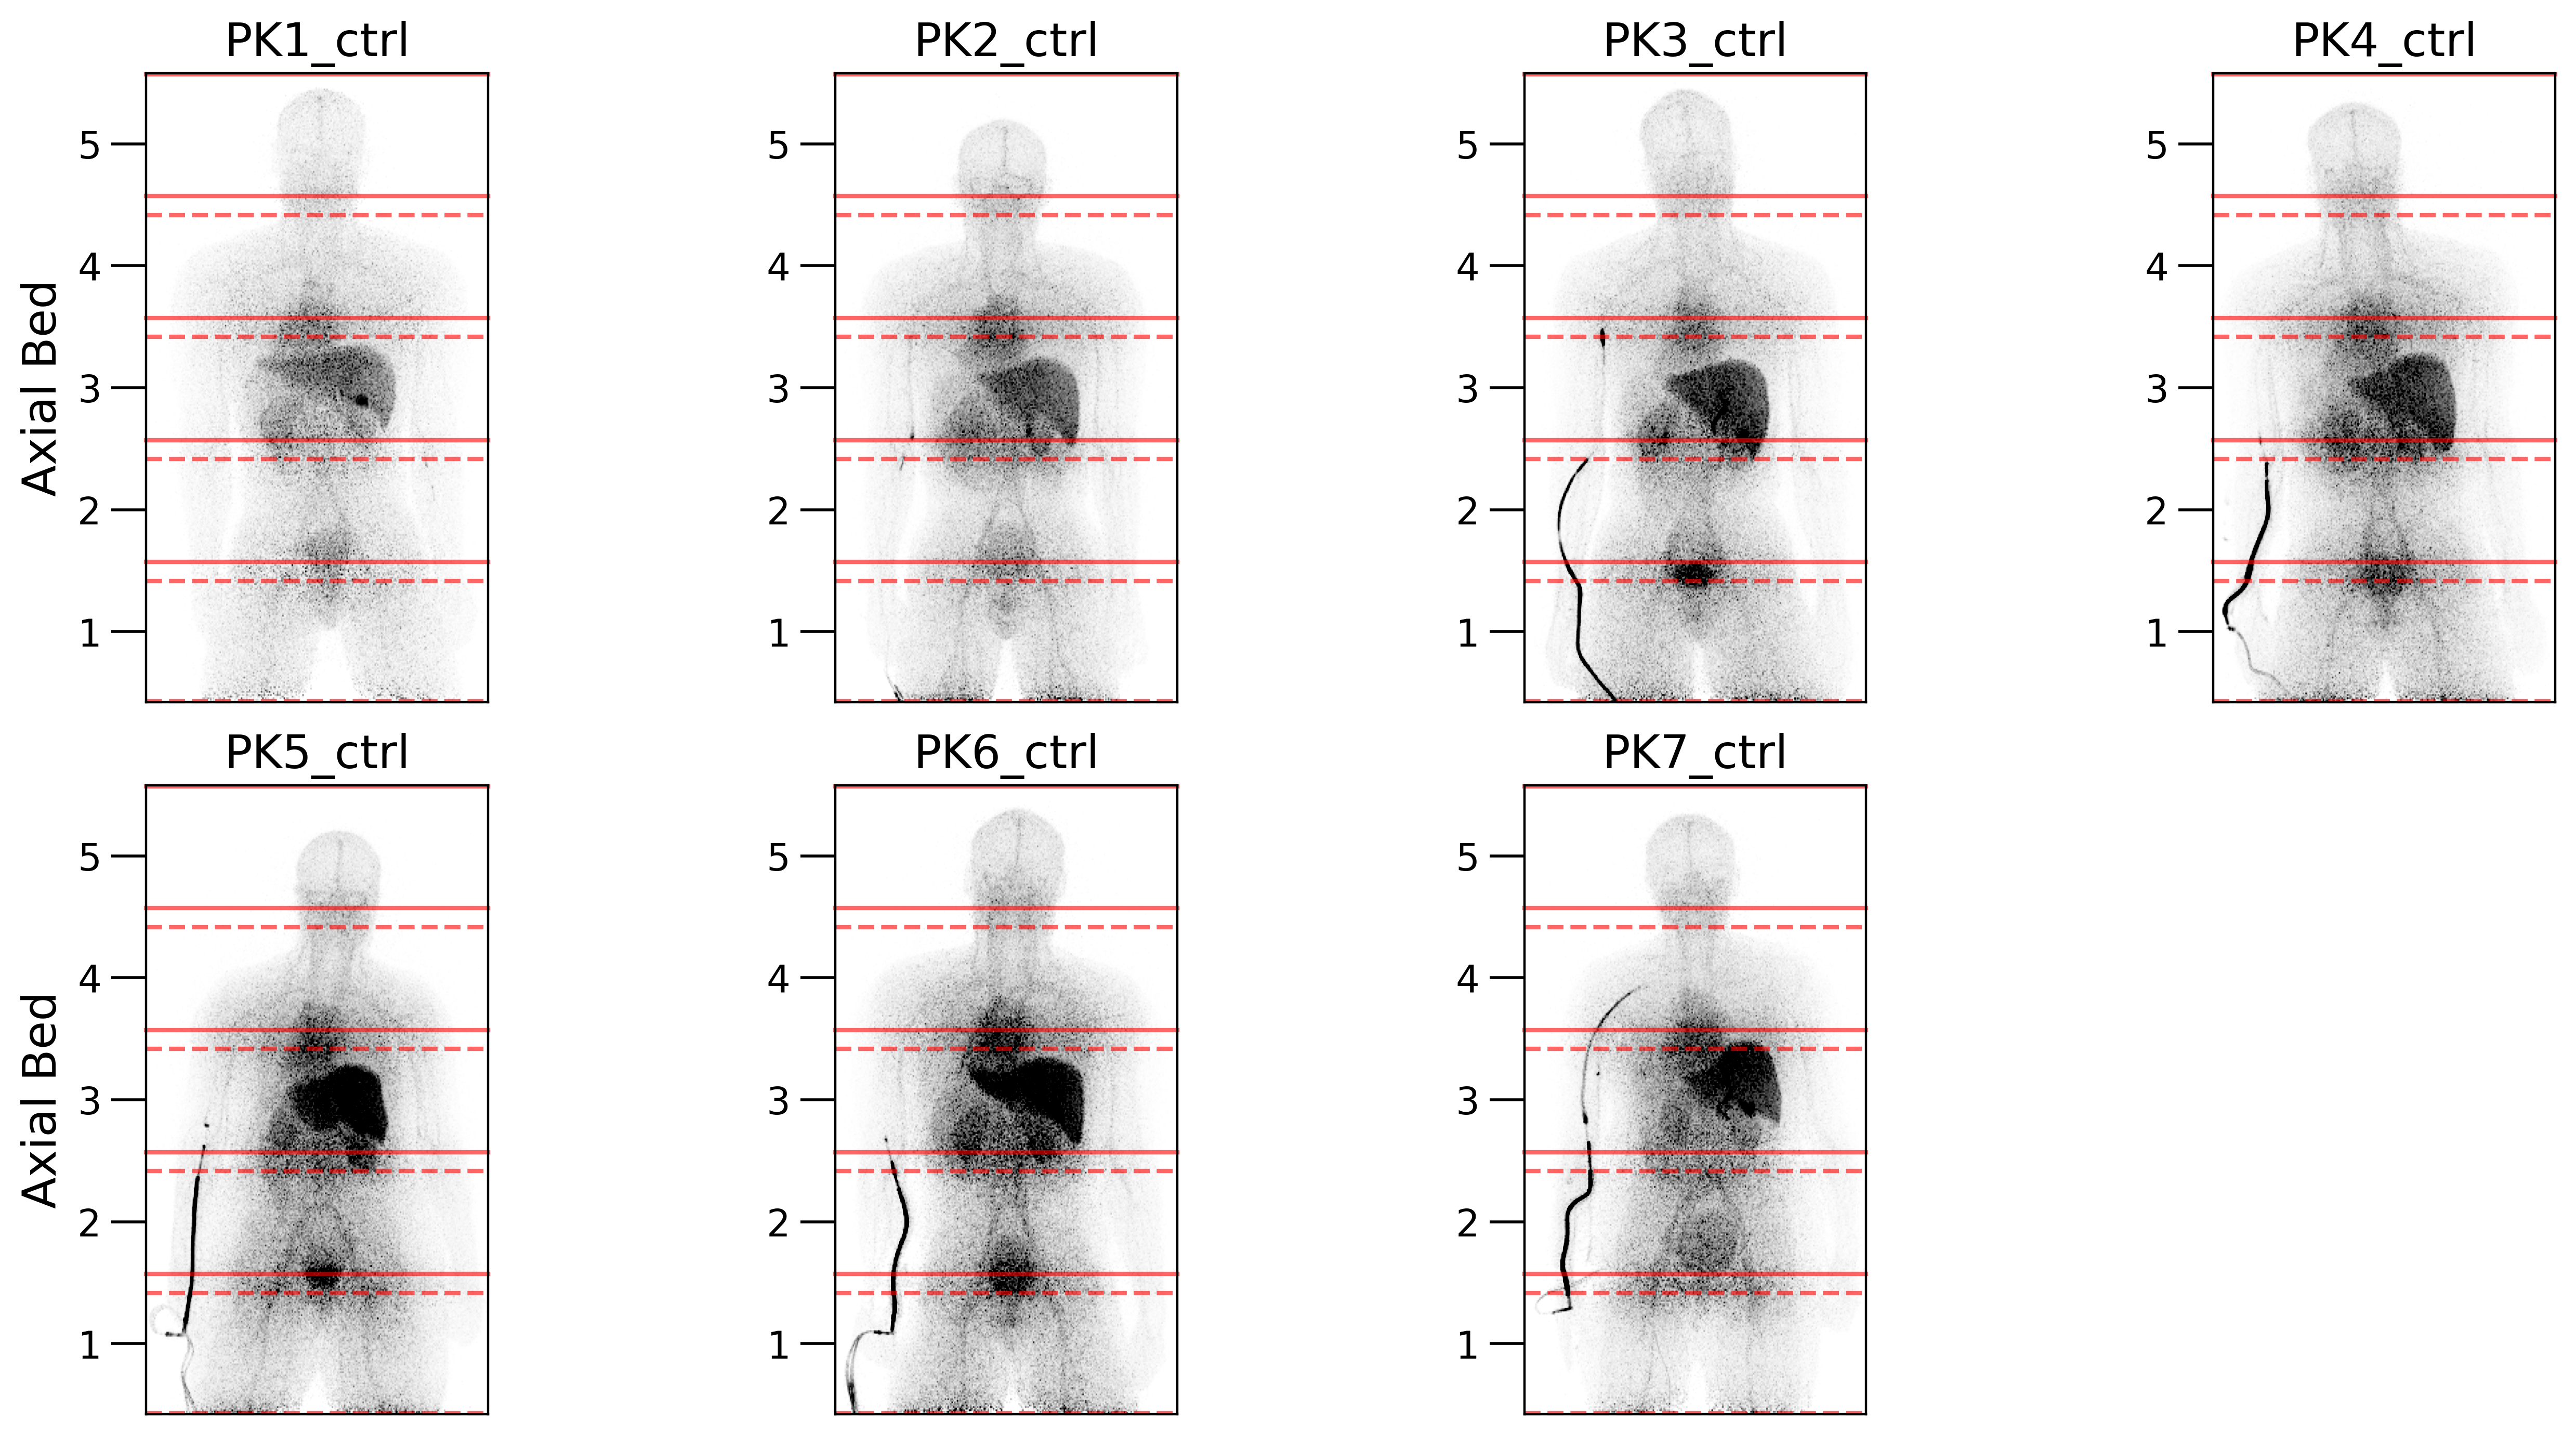
\includegraphics[scale=0.5,angle=0]{3_Results/3_1_DWB_Optimization/figures/3_1_MIPS_ctrl.pdf}
\caption{MIP projections of 7 volunteer control DWB scans with overlay of axial bed start and end location.} 
%TODO: Add over-scan in the CBM D-WB protocols. 
\label{fig3_1:ctrl_mips}
\end{figure}
%
\begin{figure} [ht!]
\centering
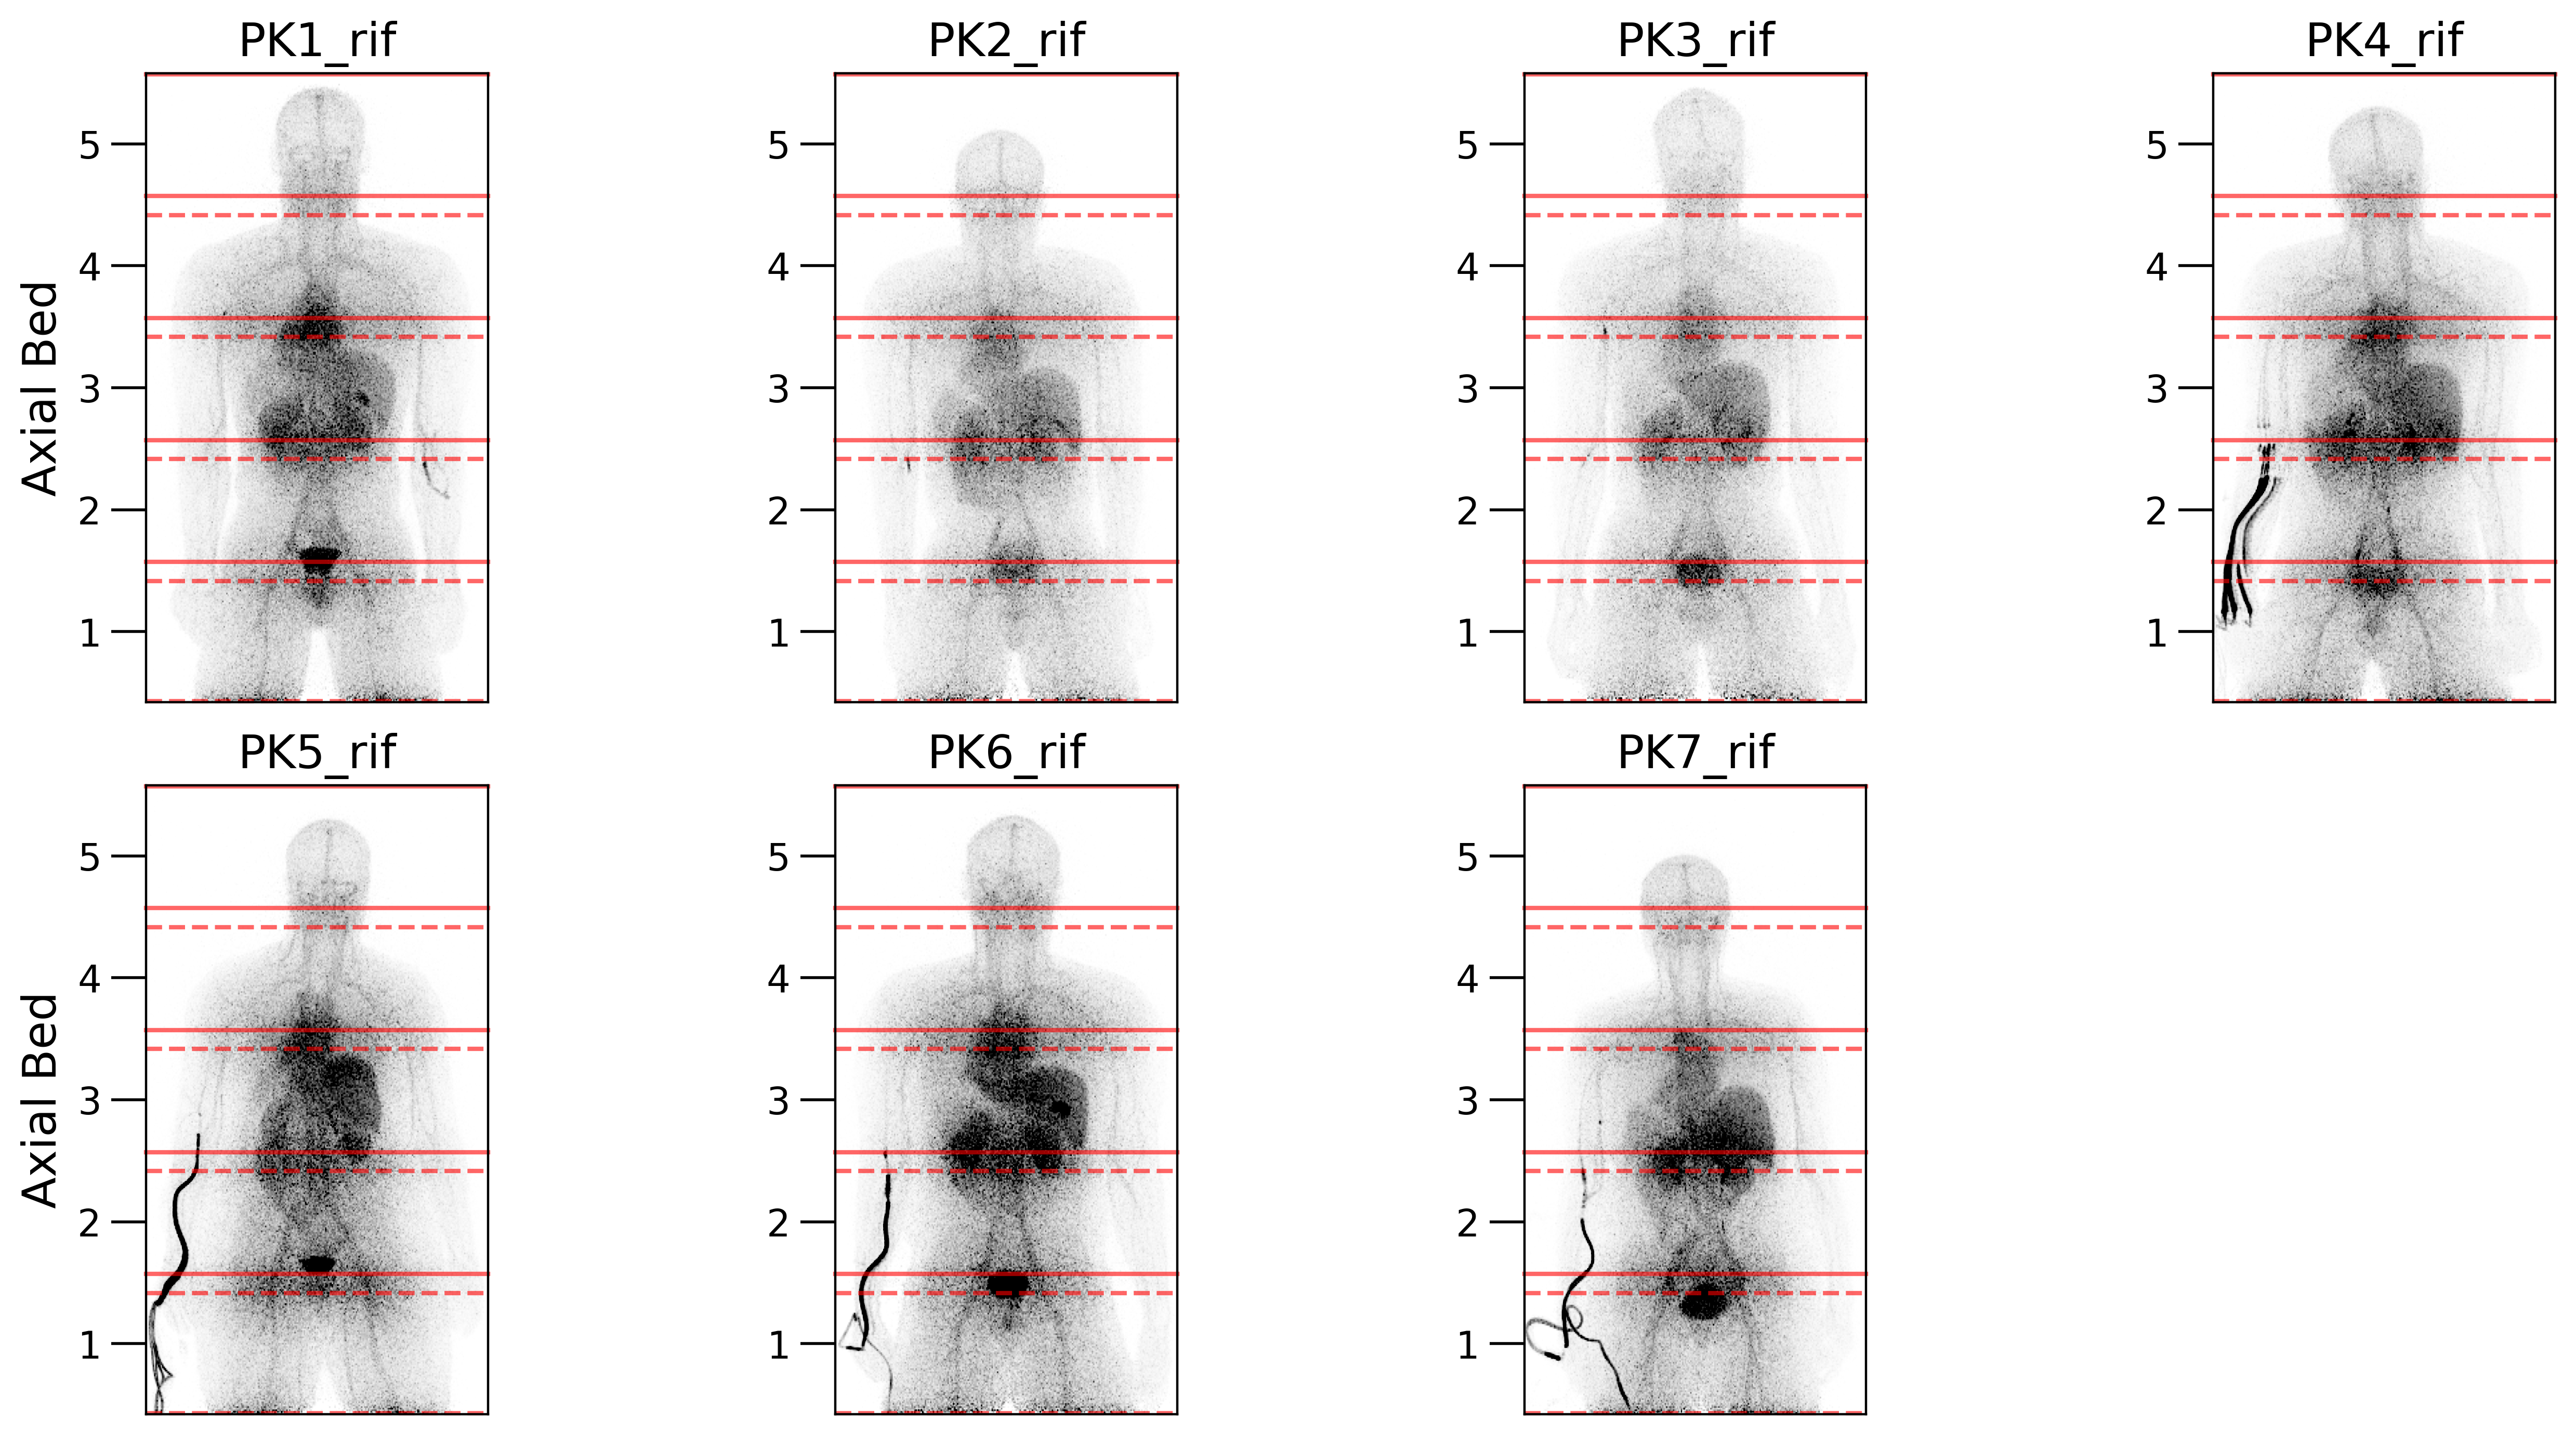
\includegraphics[scale=0.5,angle=0]{3_Results/3_1_DWB_Optimization/figures/3_1_MIPS_rif.pdf}
\caption{MIP projections of 7 volunteer rif DWB scans with overlay of axial bed start and end location.} 
%TODO: Add over-scan in the CBM DWB protocols. 
\label{fig3_1:rif_mips}
\end{figure}
%
%
%
\begin{figure} [ht!]
\centering
\includegraphics[scale=0.5,angle=0]{3_Results/3_1_DWB_Optimization/figures/3_1_BoxPlots_DTBeds.pdf}
\caption{Box plots of intra-bed delays $dl_{bed}$ of the IsotoPK DWB protocol used in practice.} 
%TODO: Add over-scan in the CBM D-WB protocols. 
\label{fig3_1:BoxPlots_beds}
\end{figure}
%
\begin{figure} [ht!]
\centering
\includegraphics[scale=0.5,angle=0]{3_Results/3_1_DWB_Optimization/figures/3_1_BoxPlots_DTSweeps.pdf}
\caption{Box plots of delay between WB Sweeps $dl_{Sweep}$ of the IsotoPK DWB protocol used in practice.}
%TODO: Add over-scan in the CBM D-WB protocols. 
\label{fig3_1:BoxPlots_sweeps}
\end{figure}
%
%
%
\section{Optimization of DWB acquisition protocol on the Signa PET-MR}
Part of this PhD project was allocated in developing a fully-automated DWB protocol on the Signa PET/MR. 
The main requirement for the envisioned protocol was to allow for continuous capture of PET data during DWB acquisition, into a single list-mode file for all bed positions. Then the data could be processed after acquisition, split to individual data for each bed position and reconstructed with the correct bed positional information. Using such an acquisition strategy the delays between bed positions and WB sweeps could be reduced to the time taken by the physical motion of the scanner table alone. 

Towards this goal, the PhD project schedule included a four week industrial secondment with GE healthcare, for the purpose of exploring tools that could enable the automation of DWB protocols. Three weeks of this secondment were spend at factory facilities of GE healthcare (Waukesha, Wisconsin, USA), %with the opportunity the gain insights on the operations of the Signa PET-MR scanner. 
There with help of the PET/MR team it was made possible to exploit in-build factory tools of the Signa PET/MR for the purposes of DWB automation. The two key tools necessary were: 
\begin{itemize}
    \item\textbf{Table Emulation} \\
    This tool allows for disassociation of the table position between the MR and PET system. It is the key tool that allows for the PET system to acquire continuously, while the MR system governs table motion. The disadvantage of this functionality is that once table emulation is enabled MR acquisitions cannot be performed while acquiring PET data.
    \item\textbf{Table Motion} \\
    This tool commands the MR system to execute movements of the scanner bed. It can be used to drive the bed to a target location at a desired speed. 
\end{itemize}

The automated DWB protocol was implemented as a Python class, because the python programming language is available on the PET/MR system's console and allowed for easy integration of the system tools with our designed routines, all under a common system clock for accurate timing of bed movements and registration of events.
The protocol was named "Auto-IsotoPK", but despite its name is a generic DWB protocol that is not limited to the IsotoPK pharmacokinetic study. It allows for an optional single-bed dynamic phase to be acquired before starting the DWB acquisition. It also allows for any number of beds to be used for DWB acquisition and positioning of the beds using for each examination using an initial MR scout image. 
Because MR acquisitions cannot be performed after \textit{Table Emulation} is enabled, all bed position MRACs must be acquired prior to the PET examination and used for all WB sweeps of the study.

A short \gls{sop} on the operation of the protocol is given in Appendix~\ref{chap:AppendixA}.

After the procedure is completed, the whole PET study is stored as a single list-mode file. The precise timing information of the acquired bed positions are saved in a log file, to be used for the post-processing procedure. 

\subsection{Results from NHP study}
After initial tests using phantoms, the protocol was tested on an actual pre-clinical DWB study. A macaque was scanned under full sedation with a novel $^{18}$F-Crizotinib tracer, that was being investigated for uses with \gls{nsclc}. The DWB study was required to examine tracer crossing of the blood-brain barrier and tracer uptake and excretion from other organs. The macaque was injected with 185 \si{\mega \becquerel} of the novel tracer. An initial dynamic phase was requested, centred over the brain for a duration of 90 s, followed by a DWB study of 3 bed positions. The study was planned for an approximate total duration of one hour. A total of 28 WB sweeps and frames per bed were fitted in the study, with the framing of 3$\times$10~\si{\s}, 5$\times$20~\si{\s}, 5$\times$30~\si{\s}, 5$\times$45~\si{\s}, 10$\times$60~\si{\s}. 
Acquisition of the required MRACs was performed prior to injection, at the planned bed positions shown in figure~\ref{fig3_1:Macaque_MRI}. In this acquisition only the body coils of the PET-MR system were used, designed for use with the human body size and load, which resulted in sub-optimal MR quality for automated estimation of attenuation maps. Attenuation maps had to be created manually in post-processing of the data to adequately correct the PET reconstruction for attenuation.  

\begin{figure} [ht!]
\centering
\includegraphics[scale=0.5,angle=0]{3_Results/3_1_DWB_Optimization/figures/3_1_Macaque_MRI.pdf}
\caption{MRAC acquisitions of NHP study showing the planned bed positions of the two acquisition phases.}
\label{fig3_1:Macaque_MRI}
\end{figure}

Following the MRAC acquisitions and after the automated acquisition protocol, the study started with the injection of the NHP subject followed by an hour of PET imaging. 
The complete study dataset was recorded in a single list-mode file, of which the head curve (curve of prompts rate with time) can be seen in figure~\ref{fig3_1:Macaque_Head_Curve}. By overlaying the recorded timing information over this curve, the two phases of the acquisition (SBD and DWB) as well as the three bed position of the DWB acquisition can be distinguished. The initial 260 second of the recorded list-data's head curve with the overlaid phases and bed positions are shown in figure~\ref{fig3_1:Macaque_Head_Curve_Phases}. 

\begin{figure} [ht!]
\centering
\includegraphics[scale=0.45,angle=0]{3_Results/3_1_DWB_Optimization/figures/3_1_Macaque_Head_Curve.pdf}
\caption{Head curve (prompts rate against time) of the acquired NHP study DWB data in a single list-mode file using the optimised protocol.}
\label{fig3_1:Macaque_Head_Curve}
\end{figure}

\begin{figure} [ht!]
\centering
\includegraphics[scale=0.45,angle=0]{3_Results/3_1_DWB_Optimization/figures/3_1_Macaque_Head_curve_Phases.pdf}
\caption{Head curve (prompts rate against time) of the acquired NHP study showing the SBD and DWB phases of the acquisition and the three DWB bed positions.}
\label{fig3_1:Macaque_Head_Curve_Phases}
\end{figure}
%
Using the timing information recorded by in the log file, the data were split into four individual bed position datasets and were processed with the GE-PET toolbox individually as single bed dynamic studies. The list-mode data along with the generated corrections were then exported into the CASToR data-file format for subsequent reconstruction tests. A \gls{mip} view of 3D reconstructions (averaged across all dynamic frames) is shown in figure~\ref{fig3_1:Macaque_PET}. \\
An image derived input function was estimated from the PET data using the right carotid VOI, which was visible on both phases of the acquisition, and the left ventricle. Both VOIs provided similar blood activity values in the DWB phase and were averaged to produce the final IDIF.
%
\begin{figure} [ht!]
\centering
\includegraphics[scale=0.45,angle=0]{3_Results/3_1_DWB_Optimization/figures/3_1_Macaque_PET.pdf}
\caption{MIP views of the NHP study's reconstructed PET images, for the two phases of the acquisition.}
\label{fig3_1:Macaque_PET}
\end{figure}
%
%
\begin{figure} [ht!]
\centering
\includegraphics[scale=0.45,angle=0]{3_Results/3_1_DWB_Optimization/figures/3_1_NHP_InputFunction.pdf}
\caption{NHP study's image derived input function using information from multiple bed positions.}
\label{fig3_1:Macaque_PET}
\end{figure}
%
Using the log timing information an estimation of the delays (time gaps) for this single NHP study using the automated acquisition protocol was made. The results showed an average intra-bed delay time $dl_{bed}$ of 3.77 s (95\%CI: 3.62,3.91) and an average delay time between sweeps $dl_{Sweep}$ of 4.6 s (95\%CI: 4.53, 4.67).


\section{Discussion}

Furthermore the hard-set bed positions do not always allow for optimum use of the effective A-FOV in each examination, as seen for example in examination PK2 in figures~\ref{fig3_1:ctrl_mips}~and~\ref{fig3_1:rif_mips}. In some cases a fewer number of bed positions might be adequate and preferable as it would lead to substantial increase of sampling frequency per bed. \\




\section{Conclusion}



%\subsection{Auto-IsotoPK: Continuous Bed Motion on the Signa PET-MR}
%The flexibility offered by the use of the automated protocol and the dedicated \"Table Motion\" tool allowed for testing the proof of concept of CBM on the Signa PET-MR scanner. Although this acquisition mode is not supported by the system, we emulated the acquisition of a single whole-body sweep by commanding a table movement at a speed of \SI{5}{\milli\metre\per\second}. The duration of the total sweep, that covered the three bed positions that were acquired in the previous DWB study and included an 50\% overscan, was ...

%\iffalse
\chapter{Developments and Advancements in Dynamic Whole Body Reconstruction}
\input{3_Results/3_2_DWB_Reconstruction/3_2_DWB_Reconstruction}
%How dynamic reconstruction was implemented in CASToR (in relation to the methods explained in the theory section). 
%Short demonstration of simulation and reconstruction using 2D example.  \\
%All the works with real data , single and multi bed.  \\ 
%The use of the Spectral model and offered advantages in pharmacokinetic studies. \\
%Residuals work. \\

\chapter{Simulation Study}
The gap paper and expand if time permits. Describe more on spectral model and $K1$ and micro-parameters comparison also. \\

\chapter{Other projects: HYBRID, CASToR etc.}
All the other projects within Hybrid ! \\
\begin{itemize}
    \item Laura's Simulation \& CNN \\
    \item Lalith's MoCo mMR Brain GAN. \\
\end{itemize}

%\fi
    
    \chapter*{Conclusions and prospects}
The objective of this thesis was to explore and assess methods for improving whole-body parametric imaging, for clinical and research pharmacological applications, using multi-bed dynamic whole body PET/MRI data.
As hybrid PET/MR scanners and the majority of other PET systems provide only a limited axial field-of-view (FOV), dynamic whole-body (DWB) protocols are used to extend the effective FOV over the required axial length. But these acquisitions come at the cost of limitations in acquisition counts and sampling frequency that degrade parametric image quality and accuracy.
Several aspects were investigated, throughout the process of DWB data acquisition to data processing and reconstruction. We largely focused on the use of dynamic reconstruction algorithms for improving the use of the PET acquired data in the estimation of activity and parametric images.

Specifically, in this project we have
\begin{enumerate}
\item Developed an optimised protocol for S\&S mutli-bed DWB acquisitions on the Signa PET/MR.
\item Evaluated and compared advanced dynamic reconstruction algorithms for whole-body parametric imaging, with focus in oncological imaging.
\item Explored the use of a direct multi-bed dynamic reconstruction framework on a real WB pharmacological study.
\item Evaluated the use of adaptive residual modelling applied in DWB data and a generic dynamic reconstruction algorithm.
\end{enumerate}

Firstly, we have worked closely with the manufacturer of the GE Signa PET/MR in methods for reducing the loss of counts and sampling frequency in DWB imaging by means of reducing delays in the acquisition process. This resulted in a custom fully-automated protocol that has shown to considerably reduce delays when applied on a real DWB study on a \gls{nhp} subject. However, approval for use of this protocol with human studies requires a more thorough review of safety measures and closer collaboration with the manufacturer. Ideally, CBM acquisition techniques should also be considered for implementation as they can contribute further towards improvements and flexibility in acquisition. 

Secondly, we made use of dynamic reconstruction for DWB parametric imaging, with focus on oncology applications of dynamic FDG PET and Patlak parametric imaging, using simulated and real data.
We proposed the use of an indirect method for DWB parametric imaging based on the spectral analysis model and dynamic reconstruction which allows for generic compartmental modelling to be used during reconstruction for temporal regularisation. While the Patlak model is limited to data after steady state conditions have been reached, this novel spectral reconstruction approach enables the use of all dynamic data in the reconstruction and offers greater modelling flexibility. Post-reconstruction Patlak parametric imaging using the regularised data of the spectral reconstruction outperformed direct Patlak dynamic reconstruction. But even this method did result in high parametric image noise when reconstruction was iterated sufficiently to ensure accurate quantification. Potentials for improvement should be examined further using additional regularisation methods to deliver acceptable parametric image noise for clinical applications and ensure accurate quantification.
%All the reconstruction methods used in this work were implemented in the open-source and fully quantitative reconstruction platform CASToR and are available in the current public release of CASToR. 
Finally, we have expanded our application of dynamic reconstruction to real data from an exploratory, first in man, WB pharmacological study. We extended the use of the dynamic reconstruction to direct multi-bed reconstruction, which enabled the use of the complete DWB dataset within a single iterative loop for dynamic reconstruction. This approach inherently handles the individual bed position data's sensitivity and timing information, notably for the bed overlapping positions where previously suggested practices made use of compromising solutions, while also allowing for the use of the DSB phase data independently of its axial position. In this type of applications, the use of spectral reconstruction is favoured as it does not impose strong assumptions on the unknown underlying kinetics. Preliminary results using VOI based analysis showed good agreement with results from 3D regular reconstruction. These applications also enabled the generation of surrogate parametric $\boldsymbol{K_1}$ maps, for relative comparison between scans.
Further comparisons with post-reconstruction parametric imaging need to be conducted to explore the reliability and additional benefits of this reconstruction approach towards accurate parametric imaging, but these were not conducted at this preliminary stage of the study.

In this application, we identified a limitation in the modelling process over the bladder, that had the potential to be the source of spatially propagating errors within the dynamic reconstruction process. 
To minimise this risk we have included an adaptive residual modelling approach within the reconstruction. This method identified and selectively corrected the model activity estimates over the poorly modelled bladder region, which provided a significant reduction of model fit errors at the cost of added noise over the entire FOV. Some optimisation advancements were made using pre-treatment of residual data, but further developments are needed for reducing the induction of noise by this approach. 

A major limitation in the application of dynamic reconstruction on WB data is motion and motion induced artefacts that affect image quality and quantification. 
In the setting of DWB imaging, complex motion exists in the PET data that ideally needs to be accounted for and corrected for within the reconstruction process. 
Many approaches for including motion correction in the reconstruction have been proposed and successfully used. But estimation of the underlying elastic motion vectors over time and over the WB is a challenging task. Moreover, the limited sampling of MR and PET in DWB acquisitions may reduce the sensitivity of many data-driven approaches for motion estimation. In our evaluations, using PET raw data and MR data from attenuation correction sequences, we were unable to use common motion estimation tools for the successful estimation of elastic motion vectors.
Recently numerous Machine Learning (ML) applications for motion estimation and correction have been proposed in medical imaging. This increasing use of ML approaches for motion estimation could lead to further developments that could be useful in the DWB motion estimation problem.

During the course of this project, the introduction of the first Total-Body PET scanner in 2018 has ignited the research interest in DWB imaging. The considerable increase in sensitivity and sampling frequency by synchronous dynamic total-body scans resulted in research projects that span from clinical applications of parametric imaging to joint estimation of complex parameters over the whole-body. These also include innovative methods using the PET TOF information for motion detection and correction.
But the availability of these systems is limited, due to the very high cost and no exclusive total-body clinical applications at this time.

More recently, extended FOV scanners became available by commercial providers with an axial FOV of approximately one meter. These offer considerably more coverage than current systems of 15-26 cm axial FOV. At this time there are two systems installed in clinics, with more underway. The greater availability of extended FOV (ex-FOV) systems will lead to more research projects of DWB imaging for clinical applications~\cite{Slart2021}. As in clinics the systems with limited FOV will still be used in the near future, there can be many opportunities for interesting comparison studies on WB parametric imaging to identify the limits of multi-bed DWB imaging with respect to synchronous DWB imaging by ex-FOV scanners.
For example, it could be envisaged that for dynamic imaging of slow processes, such as in the case of Patlak FDG, the DWB protocols on regular scanners could provide sufficient parametric image quality for clinical applications and exclusive use of ex-FOV scanners is not necessary. On the other hand, for kinetics sensitive to early fast dynamics synchronous DWB imaging from ex-FOV scanners is expected to provide strong and clear benefits.

There is a considerable research focus on the subject, from whole-body modelling, whole-body corrections and reconstruction approaches, to ML applied in whole-body image analysis. The technological advancements are going to further fuel this growth of interest, but what is left to be seen is which applications of these techniques and technologies will be predominant in future clinical and pharmacokinetic applications.

        
    \appendix
    
    
    \bibliography{bibliography.bib}
    \pagebreak

    %%%%%%%%%%%%%%%%%%%%%%%%%%%%%%%%%%%%%%%%%%%%%%%%%%%%%%%%%%%%%%%%%%%%%%%%%%%%%%%%%%%%%%%%%%%%%%%%%%%%%%%%%%%%%%%%%%%%%%%%%%%%%%%%%%%%%%%%%%%%%%%%%%%%%%%%%%%%%%%%%%%%%%%
%%%%%%%%%%%%%%%%%%%%%%%%%%%%%%%%%%%%%%%%%%%%%%%%%%%%%%%%%%%%%%%%%%%%%%%%%%%%%%%%%%%%%%%%%%%%%%%%%%%%%%%%%%%%%%%%%%%%%%%%%%%%%%%%%%%%%%%%%%%%%%%%%%%%%%%%%%%%%%%%%%%%%%%
%%% Modèle pour la 4ème de couverture des thèses préparées à l'Université Paris-Saclay, basé sur le modèle produit par Nikolas STOTT / Template for back cover of thesis made at Université Paris-Saclay, based on the template made by Nikolas STOTT
%%% Mis à jour par Aurélien ARNOUX (École polytechnique)/ Updated by Aurélien ARNOUX (École polytechnique)
%%% Les instructions concernant chaque donnée à remplir sont données en bloc de commentaire / Rules to fill this file are given in comment blocks
%%% ATTENTION Ces informations doivent tenir sur une seule page une fois compilées / WARNING These informations must contain in no more than one page once compiled
%%%%%%%%%%%%%%%%%%%%%%%%%%%%%%%%%%%%%%%%%%%%%%%%%%%%%%%%%%%%%%%%%%%%%%%%%%%%%%%%%%%%%%%%%%%%%%%%%%%%%%%%%%%%%%%%%%%%%%%%%%%%%%%%%%%%%%%%%%%%%%%%%%%%%%%%%%%%%%%%%%%%%%%
%%% Version du 23 mai 2019 (Merci à Thibault CHEVALÉRIAS (CEA) pour ses suggestions et corrections)
%%%%%%%%%%%%%%%%%%%%%%%%%%%%%%%%%%%%%%%%%%%%%%%%%%%%%%%%%%%%%%%%%%%%%%%%%%%%%%%%%%%%%%%%%%%%%%%%%%%%%%%%%%%%%%%%%%%%%%%%%%%%%%%%%%%%%%%%%%%%%%%%%%%%%%%%%%%%%%%%%%%%%%%


\label{form_last}
%%%%%%%%%%%%%%%%%%%%%%%%%%%%%%%%%%%%%%%%%%%%%%%%%%%%%%%%%%%%%%%%%%%%%%%%%%%%%%%%%%%%%%%%%%%%%%%%%%%%%%%%%%%%%%%%%%%%%%%%%%%%%%%%%%%%%%%%%%%%%%%%%%%%%%%%%%%%%%%%%%%%%%%
%%%%%%%%%%%%%%%%%%%%%%%%%%%%%%%%%%%%%%%%%%%%%%%%%%%%%%%%%%%%%%%%%%%%%%%%%%%%%%%%%%%%%%%%%%%%%%%%%%%%%%%%%%%%%%%%%%%%%%%%%%%%%%%%%%%%%%%%%%%%%%%%%%%%%%%%%%%%%%%%%%%%%%%
%%% Formulaire / Form
%%% Remplacer les paramètres des \newcommand par les informations demandées / Replace \newcommand parameters by asked informations
%%%%%%%%%%%%%%%%%%%%%%%%%%%%%%%%%%%%%%%%%%%%%%%%%%%%%%%%%%%%%%%%%%%%%%%%%%%%%%%%%%%%%%%%%%%%%%%%%%%%%%%%%%%%%%%%%%%%%%%%%%%%%%%%%%%%%%%%%%%%%%%%%%%%%%%%%%%%%%%%%%%%%%%
%%%%%%%%%%%%%%%%%%%%%%%%%%%%%%%%%%%%%%%%%%%%%%%%%%%%%%%%%%%%%%%%%%%%%%%%%%%%%%%%%%%%%%%%%%%%%%%%%%%%%%%%%%%%%%%%%%%%%%%%%%%%%%%%%%%%%%%%%%%%%%%%%%%%%%%%%%%%%%%%%%%%%%%

\newcommand{\logoEd}{ed}																		%% Logo de l'école doctorale. Indiquer le sigle / Doctoral school logo. Indicate the acronym : 2MIB; AAIF; ABIES; BIOSIGNE; CBMS; EDMH; EDOM; EDPIF; EDSP; EOBE; INTERFACES; ITFA; PHENIICS; SDSV; SDV; SHS; SMEMAG; SSMMH; STIC
\newcommand{\PhDTitleFR}{Modélisation et reconstruction d'images paramétriques du corps entier en imagerie pharmacologique TEP-IRM}	%% Titre de la thèse en français / Thesis title in french
\newcommand{\keywordsFR}{TEP, reconstruction dynamique, TEP corps entier, imagerie paramétrique} %% Mots clés en français, séprarés par des , / Keywords in french, separated by ,
\newcommand{\abstractFR}{La tomographie par émission de positons (TEP) est fréquemment utilisée pour des applications cliniques, avec une majorité des pratiques reposant sur des mesures qualitatives et semi-quantitatives. Mais l'imagerie TEP a la capacité de fournir des informations fonctionnelles entièrement quantitatives sur les processus sous-jacents explorés, grâce à l'imagerie dynamique et à la modélisation cinétique. Ces informations quantitatives peuvent être utilisées comme biomarqueurs pour des applications cliniques, en particulier pour la médecine de précision. Des protocoles avec des positions du lit multiples, dédiés à l'imagerie dynamique du corps entier (DWB), ont été développés afin d'étendre le champ de vue effectif, au prix de restrictions dans le nombre de détections et la fréquence d'échantillonnage. L'objectif de cette thèse est d'améliorer la qualité de l'imagerie paramétrique du corps entier pour les applications d'imagerie DWB sur un système hybride TEP-IRM.

Dans notre première contribution, nous avons présenté le développement d'un protocole entièrement automatisé pour l'imagerie DWB sur un système TEP-IRM clinique, qui a permis de réduire les délais d'acquisition, ce qui se traduit par une augmentation du nombre de détections et de la fréquence d'échantillonnage. Le recours à l'automatisation complète a permis d'optimiser la planification des positions des lits, en utilisant au mieux le champ de vue effectif. 

Pour la deuxième contribution, nous avons développé des algorithmes de reconstruction dynamique dans un logiciel ouvert, et évalué les avantages offerts par l'utilisation de divers modèles cinétiques dans la reconstruction de données TEP dynamiques simulées et réelles. Ces évaluations étaient focalisées sur les reconstructions de lits individuels des protocoles DWB. Dans le cas particulier de l'imagerie DWB, la reconstruction dynamique a montré des propriétés favorables pour l'exactitude et la précision des images paramétriques du corps entier, tout en fournissant des images dont le bruit est comparable à celui des protocoles dynamiques standards à position de lit unique, reconstruits avec des techniques ordinaires.

Dans notre troisième contribution, nous présentons une extension des fonctionnalités développées précédemment: la reconstruction dynamique simultanée de toutes les données multi-lits. Cette méthodologie permet l'utilisation synchrone de toutes les données d'acquisition DWB dans une seule boucle de reconstruction. La méthode a été appliquée à une étude pharmacocinétique DWB réalisée sur un système TEP-IRM. Une comparaison a été faite avec des reconstructions statiques standards suivies d'une modélisation cinétique post reconstruction. Les résultats obtenus avec les deux méthodes étaient en bon accord, sans introduction de biais sur les métriques évaluées. En outre, l'utilisation de la reconstruction dynamique a entraîné une réduction notable du bruit dans les images d’émission et paramétriques. 

Dans notre quatrième contribution, une méthode de détection et de correction des erreurs de modélisation utilisant la modélisation résiduelle adaptative a été appliquée et évaluée. Elle a montré des résultats prometteurs pour la réduction des erreurs de modélisation et leur propagation, tout en permettant la généricité dans l'utilisation des algorithmes de reconstruction dynamique.

Nos résultats ont montré que la reconstruction dynamique est nécessaire en imagerie paramétrique corps-entier pour obtenir une quantification précise et stable. De nombreuses méthodes ont été proposées dans ce projet afin d’optimiser le processus de reconstruction TEP pour l'imagerie DWB, en utilisant au mieux les données dynamiques acquises sur plusieurs positions de lit. Pour généraliser son utilisation, certaines améliorations méthodologiques doivent encore être apportées pour garantir une imagerie paramétrique fiable et sans artefact, notamment en ce qui concerne les mouvements du patient.}															%% Résumé en français / abstract in french

\newcommand{\PhDTitleEN}{Modelling and Reconstruction of \mbox{Whole Body} parametric maps in PET-MRI Pharmacological imaging}													%% Titre de la thèse en anglais / Thesis title in english
\newcommand{\keywordsEN}{PET, dynamic reconstruction, whole body PET, parametric imaging}														%% Mots clés en anglais, séprarés par des , / Keywords in english, separated by ,
\newcommand{\abstractEN}{Positron Emission Tomography (PET) is used extensively for clinical applications, with the majority of practices relying on qualitative and semi-quantitative measures. But PET imaging has the ability to deliver fully quantitative functional information of underlying imaged processes by use of dynamic imaging and kinetic modelling. That unique quantitative information can be utilised as biomarkers for clinical applications, especially in precision medicine. But clinical applications often require imaging over the whole body and the majority of clinical scanners provide a limited axial Field of View (FOV). Multiple bed position protocols for dynamic whole-body (DWB) imaging have been developed to extend the effective FOV, at the cost of considerable limitations in acquisition counts and sampling frequency. The objective of this thesis is to improve the quality of whole-body parametric imaging for DWB imaging applications on a hybrid PET/MR scanner.

In our first contribution we presented the development of a fully automated acquisition protocol for DWB imaging on a clinical PET/MR system, which resulted in reduced delays between whole body sweeps of the dynamic whole-body acquisition. These improvements can be used towards increasing acquisition counts and sampling frequency. Furthermore, the use of full automation enabled optimized planning of the individual bed positions for the best use of the effective FOV. 

For the second contribution we developed dynamic reconstruction algorithms within an existing open source reconstruction software. We evaluated benefits offered by use of various dynamic models in reconstruction, using simulated and real dynamic PET data. These evaluations were focused on reconstructions of individual beds from DWB acquisition protocols.
Our results agreed with previous findings on the use of dynamic reconstruction. In the particular case of DWB imaging, dynamic reconstruction showed desirable properties for whole-body parametric image accuracy and precision, while providing images of comparable image noise to regular single bed dynamic protocols processed with regular reconstruction techniques.

In our third contribution we present an extension of the developed functionalities on the reconstruction software for direct multi-bed dynamic reconstruction of DWB data. This methodology enables the synchronous use of all acquired DWB data within a single reconstruction loop. The method was applied on a DWB pharmacological study performed on a clinical PET/MR system and comparison was made with regular frame static reconstructions followed by post reconstruction parametric modelling. The results between the two methods were in good agreement, with no introduction of bias on the evaluated metrics. Furthermore, the use of dynamic reconstruction resulted in noticeable noise reduction in activity and parametric images.

In the fourth and final contribution, an adaptive residual modelling method was applied in reconstruction and evaluated on the DWB pharmacological study, to address modelling errors. This method showed promising results in reducing modelling errors and error propagation while also allowing for genericity in the use of dynamic reconstruction algorithms.

Overall, our findings showed that dynamic reconstruction is necessary in DWB parametric imaging to achieve accurate and stable quantification. Many methods have been proposed in this project that showed how reconstruction can be optimised for multi-bed DWB imaging, by making best use of all dynamic and bed PET raw data in the reconstruction process. But before widespread use of dynamic reconstruction, some methodological improvements need to be addressed further to guarantee artefact free and reliable parametric imaging. Most notably there is need for accurate estimation of underlying complex elastic motion in the dynamic datasets, followed by the correction of these motion types within the dynamic reconstruction process.}															%% Résumé en anglais / abstract in english

\label{layout_last}
%%%%%%%%%%%%%%%%%%%%%%%%%%%%%%%%%%%%%%%%%%%%%%%%%%%%%%%%%%%%%%%%%%%%%%%%%%%%%%%%%%%%%%%%%%%%%%%%%%%%%%%%%%%%%%%%%%%%%%%%%%%%%%%%%%%%%%%%%%%%%%%%%%%%%%%%%%%%%%%%%%%%%%%
%%%%%%%%%%%%%%%%%%%%%%%%%%%%%%%%%%%%%%%%%%%%%%%%%%%%%%%%%%%%%%%%%%%%%%%%%%%%%%%%%%%%%%%%%%%%%%%%%%%%%%%%%%%%%%%%%%%%%%%%%%%%%%%%%%%%%%%%%%%%%%%%%%%%%%%%%%%%%%%%%%%%%%%
%%% Mise en page / Page layout      
%%% NE RIEN MODIFIER / DO NOT MODIFY
%%%%%%%%%%%%%%%%%%%%%%%%%%%%%%%%%%%%%%%%%%%%%%%%%%%%%%%%%%%%%%%%%%%%%%%%%%%%%%%%%%%%%%%%%%%%%%%%%%%%%%%%%%%%%%%%%%%%%%%%%%%%%%%%%%%%%%%%%%%%%%%%%%%%%%%%%%%%%%%%%%%%%%%
%%%%%%%%%%%%%%%%%%%%%%%%%%%%%%%%%%%%%%%%%%%%%%%%%%%%%%%%%%%%%%%%%%%%%%%%%%%%%%%%%%%%%%%%%%%%%%%%%%%%%%%%%%%%%%%%%%%%%%%%%%%%%%%%%%%%%%%%%%%%%%%%%%%%%%%%%%%%%%%%%%%%%%%

\pagestyle{empty}

%%% Logo de l'école doctorale. Le nom du fichier correspond au sigle de l'ED / Doctoral school logo. Filename correspond to doctoral school acronym
%%% Les noms valides sont / Valid names are : 2MIB; AAIF; ABIES; BIOSIGNE; CBMS; EDMH; EDOM; EDPIF; EDSP; EOBE; INTERFACES; ITFA; PHENIICS; SDSV; SDV; SHS; SMEMAG; SSMMH; STIC
\begin{textblock*}{61mm}(16mm,3mm)
    \textblockcolour{white}
	\noindent\includegraphics[height=24mm]{media/ed/\logoEd.jpeg}
\end{textblock*}



%%%Titre de la thèse en français / Thesis title in french
\begin{singlespace}
\begin{center}
\fcolorbox{bordeau}{white}{\parbox{0.95\textwidth}{
{\bf Titre:} \PhDTitleFR 
\medskip

%%%Mots clés en français, séprarés par des ; / Keywords in french, separated by ;
{\bf Mots clés:} \keywordsFR 
\vspace{-2mm}

%%% Résumé en français / abstract in french
\begin{multicols}{2}
{\bf Résumé:} 
\abstractFR 
\end{multicols}
}}
\end{center}

\vspace*{0mm}

%%%Titre de la thèse en anglais / Thesis title in english
\begin{center}
\fcolorbox{bordeau}{white}{\parbox{0.95\textwidth}{
{\bf Title:} \PhDTitleEN 

\medskip

%%%Mots clés en anglais, séprarés par des ; / Keywords in english, separated by ;
{\bf Keywords:}  \keywordsEN %%3 à 6 mots clés%%
\vspace{-2mm}
\begin{multicols}{2}
	
%%% Résumé en anglais / abstract in english
{\bf Abstract:} 
\abstractEN
\end{multicols}
}}
\end{center}

\begin{textblock*}{161mm}(10mm,270mm)
\textblockcolour{white}
\color{bordeau}
{\bf\noindent Université Paris-Saclay	         }

\noindent Espace Technologique / Immeuble Discovery 

\noindent Route de l’Orme aux Merisiers RD 128 / 91190 Saint-Aubin, France 
\end{textblock*}

\begin{textblock*}{0mm}(182mm,255mm)
\textblockcolour{white}
\includegraphics[width=20mm]{media/UPSACLAY-petit}
\end{textblock*}
\end{singlespace}
\end{document}